\documentclass[10pt]{article}

% Packages
\usepackage{enumerate}
\usepackage{mathptmx}
\usepackage{hyperref}
\usepackage{helvet}
\usepackage{listings}
\usepackage[left=0.75in,right=0.75in,top=0.875in,bottom=0.875in]{geometry}
\usepackage{titling}
\usepackage{tabularx}
\usepackage{multicol}
\usepackage[explicit]{titlesec}
\usepackage{graphicx}
\usepackage{xcolor}

% Single column figure
\newenvironment{InlineColumnFigure}
{\par\medskip\noindent\minipage{\linewidth}}
{\endminipage\par\medskip}

% Caption
\newcommand{\Caption}[1]
{\vspace{0mm}\fontsize{9}{9}\textbf{Figure \refstepcounter{figCounter} 
\arabic{figCounter}: #1}}

\newcounter{figCounter}
\setcounter{figCounter}{0}

% ACM CHI Format
\setlength{\columnsep}{0.85cm}
\setlength{\parindent}{0pt}

\titlespacing{\section}{0pt}{10pt}{-\parskip}
\titlespacing{\subsection}{0pt}{10pt}{-\parskip}
\titlespacing{\subsubsection}{0pt}{10pt}{-\parskip}

\titleformat{\section}{\normalfont\fontsize{9}{9}\sffamily\bfseries}
{\thesection}{1em}{\MakeUppercase{#1}}
\titleformat{\subsection}{\normalfont\fontsize{9}{9}\sffamily\bfseries}
{\thesubsection}{1em}{#1}
\titleformat{\subsubsection}{\normalfont\fontsize{9}{9}\sffamily\itshape}
{\thesubsubsection}{1em}{#1}

\pagenumbering{gobble}

%===============================- 80 columns -=================================%
\begin{document}

% Title
\begin{center}
{\LARGE \sffamily \textbf{Course-Management System: Final Report} 
\vspace{2mm}}\\
\begin{tabular}{cccc}
\textbf{Stuart Douglas} & \textbf{Matthew Pagnan} & \textbf{Rob Gorrie} & 
\textbf{Derek Dagworthy}\\
1214422 & 1208693 & 1222547 & 1214937\\
McMaster University & McMaster University & McMaster University & McMaster 
University\\
dougls2@mcmaster.ca & pagnanmm@mcmaster.ca & gorrierw@mcmaster.ca & 
dagwordj@mcmaster.ca\\
\end{tabular}
\end{center}
\vspace{2mm}

\begin{multicols}{2}

% =================== Section =================== 
\section*{Abstract}
The final report for a design project for a course-management system is presented 
here. The proposed course-management system allows university students to enroll in courses, view their 
schedule and perform other course-related tasks from a web portal.\\

Firstly, the proposed project and suggested improvements over existing systems are explained. To inform this, four Canadian university course-management systems were surveyed, and the surveys are presented after the suggested improvements. Each survey 
has a brief description of the software followed by a critique of the major usability flaws and 
strengths. Three personas are then presented to demonstrate the potential users of the system that guided the design process. Following personas, information about the usability 
tests conducted for this system is presented followed by the results, discussion about the results, and final conclusions about the project.

\section*{Note about Formatting}
This document strictly follows the ACM CHI format. Extra spacing between paragraphs is created by LaTeX to better arrange content, and is not directly controllable by the creator. The format used for the Personas section is based off of the format given along with Milestone 2 to fit into the 2-column layout, with images included inline (which does not violate the ACM CHI template). Extreme care has been given to follow the specified format exactly, including fonts, margins, and figures.

% =================== Section =================== %
\section*{Introduction}

% =================== SubSection ================== %
The project proposed in this document is the design of a new 
university course-management system. Through scrutinization of several 
pre-existing systems, we will apply design concepts discussed in class to 
determine what features and design choices are crucial to the success of a course-
management system's design.\\

Users of the proposed system should be able to perform the following functions:
\begin{itemize}
\item enroll in courses
\item change time slots for lectures, tutorials, and labs of enrolled courses
\item view weekly schedule
\item view exam schedule
\end{itemize}

In the following section we will introduce several possible improvements that 
could be made to existing systems, informed by the system surveys conducted. These suggested improvements were incorporated into designs mockups for the new system, and into the final design of the working system.

% =================== SubSection =================== %
\subsection*{Suggested Improvements to Existing Systems}
We have outlined several improvements over existing systems that have been incorporated into the design of the new system. The software surveys identified 
several key areas of weaknesses, and solutions to those are presented below.

\subsubsection*{Dynamic Element}
One of the highlighted points of weakness in all the systems surveyed was the 
ability to surface the most relevant data to the user quickly and consistently. 
To improve this aspect, the concept of an intelligent, ``dynamic'' element was 
proposed. This prominent element is the first thing users see on the home page of the new system. Several factors including the current date and enrollment 
status are used to determine which task the user is most likely to perform.\\

For example, when the user accesses the system during exam season, the element 
 displays the student's exam schedule. During the course registration period, 
the element displays information related to course registration. If a user 
is not yet accepted into University, the element displays their application 
status.\\

This dynamic element helps users quickly find the information they are 
looking for by making information more visible and easier to access. All functions continue to be 
displayed below in a static and consistent manner, in case the user wishes to perform a less common task.

\subsubsection*{Improved Navigation}
Many tasks performed by users of course-management software are broken into 
several steps. A weakness of the existing products was in visually showing the 
user at which step they were at. To solve this, a ``breadcrumbs'' navigation element was added  when the user is engaged in a multi-step task. This element shows which step the user is currently on, and includes the ability to 
go back to a previous step, or jump ahead to the first uncompleted step.\\

This visual indicator improves the user's comprehension of how the system 
works, and gives them the ability to better navigate between steps. It also improves user satisfaction, 
as they are less likely to become impatient when they know exactly 
how many steps they have completed and how many remain. 

\subsubsection*{Smarter Schedule Generation}
An initial proposal for the system was to have the system generate several possibly schedules based on the users wishlist, and rank them based on several factors such as early classes, gaps between classes and having certain days completely off. We do believe this would be a meaningful addition to a course-management system, however decided not to include it in the final product due to time and resource constraints.

% =================== Section =================== %
\section*{Related Work}
Four course-management systems from Canadian universities were selected for 
review. For each system, a brief description was followed by a critique of 
the major usability flaws and strengths. From this, the main goals and tasks of 
users using the systems was extracted. 

% =================== SubSection =================== %
\subsection*{McMaster University -- Mosaic}
The purpose of the software is to allow students to manage their courses 
(enrolling, dropping etc.), and view information about their current status 
(current timetable, enrollment status, financial balance etc.). The main 
interface for the software consists of several collapsible modules 
encapsulating different aspects of the software in a main column. These include 
Academics, Finances, Personal Information, and Admissions. A small column to 
the right holds less common sections, such as Enrollment Dates and Graduation. 
The focus of this analysis is on two common tasks -- enrolling in courses and 
viewing one's course schedule.

\subsubsection*{Critique}
The largest usability flaws in Mosaic center around difficulty to access 
required information. Combined with an unintuitive and inconsistent navigation 
interface. The HTA for enrolling in a course (appendix: Figure XXX) demonstrates this 
through the large number of steps required to perform a routine and common task. 
Other functions are hidden behind dropdown menus, and are difficult to discover.\\

The navigation is separated into a top navigation bar separated by user-type 
(e.g. Students and Employees). Within the student center page, functions are 
separated into modules, an effective strategy to group related functions. 
Navigating to one of the sub-functions (such as enrolling in a course) presents 
secondary and tertiary menus below the main one. Navigation within one of these 
is handled by blue text hyperlinks back to previous pages. Native back and 
forward browser functionality does not work. There is little visual indication 
of where the user is beyond the navigation bars at the top, which do not go to a 
depth sufficient to cover all pages used when performing common actions, such as 
enrolling in a course.

% =================== SubSection =================== %
\subsection*{Guelph University -- WebAdvisor}
Guelph University's course enrollment software, WebAdvisor, provides a variety 
of functions for students to manage their courses. The student page interface 
contains two columns -- a main column with course-related news, and a righthand 
column with links to each of the functions (Register for Courses, View Schedule 
etc). These ``function'' pages are one column, and may contain several sub-pages 
as processes are broken into steps. Navigating between sub-pages is done using 
native browser back and forward buttons. If an error occurs, such as no courses 
found for specific search criteria, a large box is displayed with information 
about the error and the option to search for a solution.

\subsubsection*{Critique}
There are a variety of usability issues associated with \mbox{WebAdvisor} that 
could be improved upon, especially in the area of navigation. There are also 
certain strengths to the system as compared to others surveyed. The navigation 
issues largely stem from a lack of consistent navigation elements to show the 
user where they are. For example, when enrolling in a course there are several 
steps that must be completed (appendix: Figure XXX). The user is not aware how many steps there are total, how many they 
have completed or how many remain. Another large usability issue is an 
inefficient use of space on the main page. The visibility of important functions 
is reduced by putting all functions in a small column to the right of the main 
content. This main content contains news items, such as exam period times and 
service outages, generally information that the user is less likely to need than 
the functions beside it.\\

WebAdvisor does do some things quite well from a usability perspective however. 
One of the most common tasks is enrolling in a course, and WebAdvisor has the 
most streamlined process of all universities surveyed. Although it is not always 
clear at which step the user is at as discussed above, the process is 
straightforward and contains much fewer steps than performing a similar task 
using a different system.

% =================== SubSection =================== %
\subsection*{Carleton University -- Central}
Central is the course-management system for Carleton University. It has a 
similar feature-set to the other systems surveyed. This includes allowing users 
to enroll in courses and view their schedule. The user interface for Central 
primarily is based on text links to different pages, with very little use of 
icons or colour. The main student page is a one-column list of text links to the 
various student-related categories of functions. A tab bar at the top lets the 
user switch between different sections of the system including Student Services 
and Employee Services.

\subsubsection*{Critique}
There are a large number of prominent usability flaws in Carleton University's 
course-management system. Visibility of common functions on the main 
page is very low, as a long list of hyperlinks contains all the categories (e.g. 
Registration, Student Records etc) requiring the user to read each one until 
they find the correct one. Once a category is selected, then another list of 
hyperlinks to each of the functions in that category is shown. 
Again, the user must read through each one until they find the desired function.\\

Another large usability flaw is the poor mapping between many actions. For 
example, when adding a course, the user first enters a course number into one of 
several (unlabeled) input boxes, and then they click the Submit button (appendix: 
Figure XXX). The submit button is aligned with other buttons for Class Search, 
which takes the user to a separate page, Reset, which undoes their changes, and 
Return to Worksheet which navigates the user to a page showing them their 
preferred courses. These buttons are not all related, and grouping them together 
may confuse the user.\\

Overall, Central is a relatively unintuitive system, requiring users to spend 
more time finding the information they need through poor mappings and a lack of 
a visual hierarchy.

% =================== SubSection =================== %
\subsection*{Waterloo University -- Quest}
The Quest system is designed to let students manage several aspects 
of their university enrollment, such as course management, financial inquiries, 
and contact information. Students can also sign up for a GO Bus pass, view their 
grades and transcript, and check the status of scholarships and other 
applications. The main page is broken up into 8 collapsible sections, 4 main 
sections (Academics, Finances, Personal Information, Admissions) with another four 
sections in a sidebar (Holds, Finance Information, Academic Information, Other 
Useful Links). The critique will focus on enrolling in courses and viewing a 
user's course schedule.

\subsubsection*{Critique}
Quest has some major usability issues when it comes to providing the user to 
information and functions they can use. The system is notorious for hiding 
options and menus from the user, requiring several screens of drill down menus 
before being able to access any meaningful options. The menus look unfinished or 
poorly formatted, and it is easy to become lost and confused while navigating 
the various pages. Navigation on the main page uses hyperlinked text, 
while traversing the deeper options is done using blue menu tabs. Native browser 
back and forward commands generally work as expected, which makes navigation a 
little more manageable. 

\section*{Personas}
Presented are the personas used to develop our design.These personas were based off of the \emph{Persona Template} as linked from the assignment outline from McMaster University, COMP SCI 4HC3 These personas were created to archetype the most common user types, and have been integral to developing a product that will satisfy all of them.\\

%%============================= Persona 1 ======================================%
\subsection*{Trevor Clark}
\begin{center}

\includegraphics[width=50mm]{images/Trevor.jpg}\\
\Caption{``When do classes start?"}
\end{center}

\begin{itemize}
\item Born: London, ON
\item Age: 22
\item 3rd Year Engineering Student at McMaster
\end{itemize}

Trevor is a third year Civil Engineering student at McMaster. He currently lives 10 minutes away from campus with some friends he met in first year. Trevor's parents are paying for his tuition and he has a student loan which he uses to pay for rent and food.\\

Trevor is unorganized and rarely goes to class. He also forgets to hand in assignments on time. Trevor is not a part of any clubs and prefers to spend his free time with his housemates playing video games.\\

Trevor has trouble remembering important dates, like his course selection or when his exams are. When he searches for information, he usually gives up after five minutes if he cannot find what he is looking for. Trevor would like it if the new course management system was quick and easy to use. He also would not mind it if certain information was made more accessible during certain times of the year (easy to see link to exam schedule around exam season).

%%============================= Persona 2 ======================================%
\subsection*{Candice Smith}
\begin{center}

\includegraphics[width=70mm]{images/Candice.jpg}\\
\Caption{``I don't know what electives I want to take for university next year"}
\end{center}
\begin{itemize}
\item Born: Oakville, ON
\item Age: 18
\item Grade 12 High School Student
\end{itemize}

Candice has been accepted to the chemistry program at McMaster. Candice currently lives at home with her parents and will be moving into residence in the fall. Her parents are paying for her tuition, but Candice is paying for her residence and meal plan. Candice works part time at the Fortinos in her home town to save up money so she can go to the movies whenever new movies come out.\\

Candice has done well in all of her classes in high school and is a part of several high school groups; such as the volleyball team, track and field team and the Harry Potter fan club.\\

Candice has several electives that she can take, but she cannot decide which ones to enrol in. She has heard that she can change courses during the first couple weeks of class and plans on doing that if she ends up changing her mind. Candice has already made a list of classes she would like to take in her first year and is waiting for the course registration to open up. Candice would like the new course management system to allow her to browse all the courses available to her and would like it if there were descriptions for each course that she could read before she registers.

%%============================= Persona 3 ======================================%
\subsection*{Adrian Lopez}
\begin{center}

\includegraphics[width=70mm]{images/Adrian.png}\\
\Caption{``I have a lot of new things to get used to in Canada"}
\end{center}

\begin{itemize}
\item Born: Mexico City, Mexico
\item Age: 20
\item 2nd Year Geography Student on Exchange to McMaster
\end{itemize}

Adrian is a geography student from Mexico on exchange at McMaster for the year. Adrian is living in a house 20 minutes away from campus with other students in the foreign exchange program. Adrian's tuition is being paid for by a grant he received for being a part of the foreign exchange program. His parents are giving him some money for rent and food but Adrian has to pay for some of it himself. Adrian is a hard working individual during the week and can be found in the Thode library between classes. Adrian likes to get all of his assignments done during the week so he can spend his weekend going to clubs with his housemates and friends.\\

Adrian is a part of the improv club which he regularly goes to. Adrian has chosen a light course load this year as he would like some time to experience Canada before he goes back to Mexico next September.\\

Since English is not Adrian's first language he sometimes has trouble reading and understanding websites that are primarily text, and he can get confused while navigating to the information he is looking for. Adrian would like it if the new course management system was easy to navigate and intuitive enough that he doesn't need to read an instruction manual to know how to use it.

% =============================== USABILITY =========================== %
\section*{Design Mockups}
Please refer to the appendix for final design mockups of each screen. They were closely adhered to when developing the system, as can be noted by examining the screenshots from the new system at the end of the appendix.

% =============================== USABILITY =========================== %
\section*{Usability Tests}
\subsection*{Overview}
This section of the document describes a plan for conducting a usability test for our course management software. This usability test plan will be based off of the \href{http://www.usability.gov/how-to-and-tools/resources/templates/usability-test-plan-template.html}{\underline{Usability Test Plan Template}} created by the U.S. Department of Health \& Human Services. The goals of this usability test are to establish a baseline of user performance, establish and validate user performance measures, and identify potential design concerns to be addressed in order to improve the efficiency, productivity, and end-user satisfaction of the product.\\

The usability test objectives are:
\begin{itemize}
\item To determine design inconsistencies and usability problem areas within the user interface and content areas
	\begin{itemize}
	\item Navigation errors: failure to locate functions, failure to follow recommended screen flow
	\item Presentation errors: failure to locate and properly act upon desired information in screens, selection errors due to labeling ambiguities
	\end{itemize}
	
\item Exercise the web site under controlled test conditions with representative users. Data will be used to access whether usability goals regarding an effective, efficient, and well-received user interface have been achieved.

\item Establish baseline user performance and user-satisfaction levels of the user interface for future usability evaluations.
\end{itemize}

\subsection*{Procedure}
The following details about the usability tests are sufficient data for others to replicate the tests in a consistent manner.
 
\subsubsection*{Test Conditions}
The participant's interaction with the application will be monitored by the facilitator seated in the same room. The facilitator will be responsible for taking notes and logging data during the tests. All tasks will be run on the same machine, using the same web browser. The machine will be a desktop computer running Windows or Mac OS X. The browser used will be either Safari (7 or later), Chrome (39 or later), or Firefox (29 or later).

\subsubsection*{Task Setup}
The facilitator will initially explain that the amount of time taken to complete the test task will be measured as well as how many errors were made and other notes about the participant's interactions with the software.\\

Before each task, the facilitator will ensure that no courses are enrolled in by navigating to the system's enroll page and dropping all current courses. The facilitator will then navigate to the home page of the system. The facilitator will instruct the participant to `think aloud' so that verbal record exists of their interaction with the application. Then, they will  inform the participant of the task's objective, and allow the participant to control the computer.

\subsubsection*{Task Procedure}
As soon as the participant starts the task the facilitator will begin to time the participant. The facilitator will observe and enter user behaviour, user comments, and system actions. After the participant has completed all tasks they will be asked to complete a 14-question questionnaire (see Appendix: Table 1) using a 5-point Likert scale with 1 being \emph{very easy} and 5 being \emph{very hard}.

\subsubsection*{Tasks}
Following is a list of the tasks the participant will complete. Note: the reason the courses in tasks 1.1 and 2.1 are different is that dummy courses were used for the new system, and have different course codes.
\begin{itemize}
\item \textbf{Task 1.1} - Have user enroll in the following courses for the \emph{Winter 2016} term through Mosaic, selecting lectures, tutorials, and sections so as to eliminate conflicts as needed:
\begin{itemize}
\item ANTHROP 1AA3
\item ANTHROP 1AB3
\item COMPSCI 2DM3
\item BIOLOGY 1A03
\end{itemize}
\item \textbf{Task 1.2} - Have user find their exam schedule for the Fall 2015 semester on Mosaic 
\item \textbf{Task 1.3} - Have user find their weekly schedule for the Fall 2015 semester on Mosaic
\item \textbf{Task 2.1} -  Have user enroll in the following courses using the new system selecting lectures, tutorials, and sections so as to eliminate conflicts as needed:
\begin{itemize}
\item ANTHROP 4AA3
\item ANTHROP 4M03
\item COMP SCI 1TA3
\item BIOLOGY 2AA3
\end{itemize}
\item \textbf{Task 2.2} - Have user find their exam schedule for the Fall 2015 semester using the new system
\item \textbf{Task 2.3} - Have user find their weekly schedule for the Fall 2015 semester using the new system
\end{itemize}

\subsection*{Success Metrics}
Success metrics refers to user performance measured against specific performance goals necessary to satisfy usability requirements. Scenario completion success rates, error rates, subjective evaluations, and scenario completion times will be used.

\subsubsection*{Scenario Completion}
Each scenario will require that the participant performs a specific, common task. The scenario is complete when the scenario's goal has been obtained or the participant requests sufficient guidance to warrant scoring the scenario as a critical error, at which point the facilitator will terminate the task.\\

The goal for scenario completion is that the participant successfully completes the task to completion.

\subsubsection*{Errors}
Errors are deviations from the target behaviour necessary to complete the scenario. Participants may or may not be aware that the they have deviated from the target behaviour. Errors may be procedural, in which the participant does not complete a scenario in the most optimal means (e.g. excessive steps and keystrokes). These errors may also be errors of confusion (such as attempting to edit an un-editable field).\\

The goal for errors is for the new system to have at most the same number of errors for each task as the old system. Optimally, some (if not all) tasks will have less errors than the old system. It is important to note that some participants may have experience using Mosaic, and so will make less errors. Even if this is the case, the goal remains the same as we are performing tests to see if a replacement system would be an improvement, in which case the current system would have the advantage of most users having experience.

\subsubsection*{Subjective Evaluations}
Subjective evaluations regarding ease of use and satisfaction will be collected via questionnaires, and during debriefing at the conclusion of the session. The questionnaire will utilize a 5-point Likert scale, and will ask participants their perceived ease-of-use of a variety of functions and features. Each question will be asked once for Mosaic, and once for the new system.\\

The subjective evaluation goal is to have an average response number across all participants and all questions that is at least 1 point higher on the Likert scale for the new system, as well as to have no questions with an average response for the new system more than 1 point below the response for the same question for Mosaic. This ensures that the overall experience is significantly better from a user standpoint, and there are no areas of particular weakness with the new system.

\subsubsection*{Scenario Completion Time}
For each scenario to be tested, the time it takes the participant to complete the scenario will be recorded, to the nearest second. This time begins as soon as the user starts the task, and finishes as soon as the task is completed. If the task is not completed, the time is not recorded and the result is noted in the errors section.\\

The goal for scenario completion time is to have the average completion time of each task be at most 10\% slower on the new system, and the total completion time for all tasks on the new system to be at least 20\% less than with Mosaic. This ensures that no task is significantly slower with the new system, and the overall benefit of the new system is significant.

\section*{Results}
The above usability tests were conducted with 8 different participants, all of whom had some experience using Mosaic. All participants were students at McMaster University.\\

After analysis of the intersystem task results and the questionnaire results, several conclusions can be drawn. Both the questionnaire and the test tasks reflected a nearly ubiquitous distinction between the subjective usability of the two systems (Mosaic and our newly implemented system).

\subsection*{Scenario Completion}
All participants successfully completed all scenarios in both Mosaic and the new system.

\subsection*{Errors}
There were two errors in the new system that were very common during the tests. When users were first asked to enroll in a course, they navigated to the Enroll from Wishlist page, and spent several moments trying to find out where to go next (the page stated that their wishlist was empty). The other common error was when users were selecting criteria to search for courses. The two dropdowns for course level and course code were designed to be mutually exclusive, however a majority of users first selected a course level, and then selected a course code (blanking out their course level choice). There were significantly more errors using Mosaic, our success metric was met.

\subsection*{Subjective Evaluations}
Very clear distinctions could be observed between the two systems in terms of subjective ease-of-use, as was found in the questionnaire results. Participants each recorded the difficulty of completing a handful of tasks on Mosaic, and then the difficulty of completing the same tasks on the new system. The average difficulty for Mosaic tasks was recorded at 3.5 (on a 5-point Likert scale, with 5 being most difficult, 1 being most easy) whereas the new system scored an average difficulty of 1.4 (see Figure XXX). This satisfies our first success metric for subjective evaluation. The second success metric is also met (see Figure XXX) as there were no tests that had an average score at least 1 point lower on the new system.

\subsection*{Scenario Completion Times}
The most notable distinction recorded is in the consistency of enrollment time between the two systems. During the task of enrolling in a course on Mosaic, participants ranged in completion times from 0.7 to 5.53 minutes. The standard deviation for time spent enrolling in a class on Mosaic was roughly 1.6 minutes. Alternatively, the same task on the new system had completion times ranging from 1.02 to 1.68, and a standard deviation of only 0.2 (see Figure XXX). The completion times satisfied both success metrics, as the average time for each task for the new system was never more than 10\% slower than Mosaic, and the total average time was at least 20\% better than in Mosaic (see Figure XXX).\\

It can be observed, then,  that amongst the participants tested there is qualitative and quantitative  data suggesting higher usability for the new system. The new system is found to be both easier to use and more efficient than Mosaic.

\section*{Discussion}
The results of the usability tests will now be discussed in terms of the positive and negative aspects of the new systems, where it could be improved in the future, and how the results relate to the original goals of the project.

\subsection*{Positive Aspects of New System}
The results shown above show that the new system was consistently preferred by participants over Mosaic. This can be seen in the questionnaire results, with a consistently higher rating for the ease-of-use of functions in the new system over Mosaic. It can also be seen more objectively by examining the significant improvements to scenario completion time as in Figure XXX.\\

There were several particular areas of strength for the new system as noted by comments from participants and ongoing evaluation by the facilitators as they worked on the tests. Each of these strengths will now be discussed, as well as how best to incorporate them going forward.

\subsubsection*{Accessing Features from Home Page}
One of the largest complaints with Mosaic was the difficulty in finding common features such as a user's exam schedule. The improved navigation of the new system significantly reduced the time it took participants to find features, even though all participants had experience with Mosaic and no experience with the new system. Providing large, accessible buttons as well as a prominent dynamic element (see Introduction: Suggested Improvements) for the most common functions on the home screen allows the user to quickly find what they are most likely to need. Improved navigation was one of the main focuses of the new design, and the results demonstrate that the focus was an important factor in improving efficiency and user-satisfaction.

\subsubsection*{Visualization of Course Times}
During the usability tests, most participants did not acknowledge Mosaic's course times when searching for courses. They instead chose the first available lecture and tutorial and added the course to the wishlist, resolving conflicts when actually enrolling. In the new system, the lecture, tutorial, and lab times are shown directly in the search results in a visual manner (Appendix: New System -- Screenshots). The same visual structure is used when enrolling in courses, and as a result most participants were able to quickly understand why a course had a conflict and how to fix it.

\subsubsection*{Navigation Between Enrolling Steps}
The ``breadcrumb'' navigation pattern was initially added to the course enrollment pages so that a user can quickly switch between searching for courses, seeing the results, and enrolling in courses. This proved to be an effective pattern, and almost every single participant used the element as the primary way to navigate between pages when enrolling in courses. Mosaic does not have a similar element, and it was noted during the tests that many users would add one course to their wishlist in Mosaic, return back to the home page, and then navigate back to the search courses page. It was our goal to eliminate this inefficiency with the new system, and the results of the completion time tests for enrolling in courses show that it was achieved (see Figure XXX).\\

Although we have outlined the above features, there were a variety of other, less prominent enhancements that were appreciated by the participants during the tests. These included a less-cluttered UI, more obvious calls to action (i.e. bright green buttons), simpler conflict management (see Figure XXX), and an improved weekly schedule (courses colour-coded, rows all have consistent height).

\subsection*{Negative Aspects of New System}
Although the overall results from the usability tests were very positive, there were two main areas of weakness, where participants consistently encountered errors. Both areas would be primary areas of focus for future iterations.

\subsubsection*{Selecting Search Criteria from Dropdowns}
One of the design decisions for the new system was to allow the user to select \emph{either} the course level for a given subject when searching or the specific course code for the subject. The reasoning behind this was that the user would be able to quickly see all courses for a given subject and year, or they could manually choose one if they knew the code. In reality, participants consistently chose the course level and then without clicking search, would choose the course code, blanking out the course level dropdown. The design attempted to mitigate this with a large ``OR'' label between the dropdowns, and a bright green highlight for the selected one, but participants continued to make the error.

\subsubsection*{Initially Enrolling in Courses}
Task 2.1 asks the user to enroll in several courses. The initial action by almost every user was to click the ``Enroll/Drop'' button on the main page, taking them to the page for enrolling in courses from the wishlist. Two large boxes are shown saying that they are not enrolled in any courses and their wishlist is empty, but there is no indication on how to add courses. Most participants looked around and eventually found the ``Search Courses'' button in the breadcrumb navigation at the top.\\

The above two areas of weakness led to the vast majority of errors during the usability tests for the new system, and mitigating them should be prioritized for future iterations.

\subsection*{Future Improvements}
When designing future versions of the software, there are several important improvements that could be made, as can be seen in the results.\\

Improving the two weaknesses discussed above should be prioritized. For the search criteria dropdowns, the design should not require the two options to be mutually exclusive. Instead, selecting a level should filter the number of course codes available in the course code dropdown. If the user does select a course code, there should be an option to quickly add the course to the wishlist without leaving the search criteria page. This will improve the time for enrolling in courses if the user knows which courses they would like to enroll in. To improve the initial enrolling steps, a large prominent call to action from the enroll page should be shown if the wishlist is empty, pointing the user to the ``Search Courses'' page. As soon as a course is added to the wishlist, the link would disappear.\\

Another future improvement to the system would be to include the smarter schedule generation feature as discussed in \emph{Introduction: Suggested Improvements}. This would improve the process for selecting time slots, and would increase user satisfaction, as it will reduce the effort to create a schedule, while improving the schedule quality.

\subsection*{Comparison with Original Goals}
The original goal of this project was to create a university course-management system that is easier to use, smarter, and more efficient than existing systems. To create our design, we applied well-known design principles such as visibility (green buttons), mappings (course times shown on days of week table), and good conceptual models (breadcrumbs to show step-by-step nature of enrolling). The results from the usability tests clearly demonstrate that there are major usability issues with the current system (see Figure XXX), and that are new system improves upon many of the usability aspects (see Figure XXX). All success metrics were met or exceeded, demonstrating that the proposed system is a viable foundation for a new course-management software system.

\section*{Conclusion}
We proposed a design for a new university course-management system with several new features and enhancements to reduce the amount of time it takes for students to perform common tasks. We then surveyed and critiqued four existing university course-management systems, and used this information to inform our design proposals. Personas were then created to demonstrate potential users of the system and were used to guide the design process. This process involved an iterative process of design for each of the pages of the system, which resulted in a set of mockups (appendix: \emph{New System -- Final Design Mockups}) using a consistent design language and incorporating the improvements outlined earlier.\\

The mockups were used to create a working prototype of the system, implemented using common web technologies. A database of ``dummy'' courses was created to test a variety of features, and edge cases were closely examined to ensure consistent behaviour.\\

After development of the new course-management website was finished, several usability tests were created to gather data on the effectiveness of the new system compared to Mosaic. The responses from the questionnaire show that users overwhelmingly preferred the new system over Mosaic in terms of user experience. The scenario completion time results showed similar times for finding weekly schedules and consistently lower times for finding exam schedules (in some cases significantly so). The most improved task in terms of completion time however was enrolling in courses, with times improving by large margins in all trials.\\

Some potential problems identified through our usability tests are the poor visibility of the exclusive nature of the dropdowns in the search page, and the lack of instructions on the enroll page when no courses are added yet.\\

The system is clearly not a replacement for Mosaic -- it implements a small subset of Mosaic's functionality -- however, the results of the usability test and the software surveys show a need for improvement in university course-management software. The conclusion of our usability study is that the proposed system makes significant improvements over the current system and is a reasonable starting point for future changes.

\end{multicols}

\newpage
\section*{Appendix}
% ================== SUBSECTION ============================ %
\subsection*{Usability Tests -- Results}
\begin{table}[h]
\centering
\caption{Usability Questionnaire Questions (5-point Likert scale)}
\begin{tabular}{cllllllllllllll}
\hline
Question \# & With Mosaic, how easy is it to...\\\hline
Q1 & find classes for enrollment?\\
Q2 & add classes for enrollment? \\
Q3 & find your weekly schedule\\
Q4 & navigate your weekly schedule\\
Q5 & select tutorial, lecture, and lab times for your course\\
Q6 & enroll in courses\\
Q7 & resolve schedule conflicts\\\hline
\multicolumn{2}{c}{\emph{Questions 8 through 14 are identical to 1 through 7, but with the new system instead of Mosaic}}\\
\hline
\end{tabular}
\end{table}

\begin{table}[h]
\centering
\caption{Usability Questionnaire Results (5-point scale, lower is better)}
\begin{tabular}{cllllllllllllll}
\hline
Participant \# & Q1 & Q2 & Q3 & Q4 & Q5 & Q6 & Q7 & Q8 & Q9 & Q10 & Q11 & Q12 & Q13 & Q14\\\hline
1 & 5 & 4 & 2 & 3 & 3 & 4 & 5 & 2 & 1 & 1 & 1 & 1 & 1 & 2 \\
2 & 4 & 4 & 2 & 2 & 2 & 4 & 3 & 2 & 3 & 1 & 1 & 1 & 3 & 2 \\
3 & 4 & 3 & 4 & 4 & 2 & 3 & 5 & 1 & 1 & 1 & 1 & 1 & 2 & 1 \\
4 & 4 & 4 & 5 & 4 & 3 & 4 & 4 & 2 & 1 & 1 & 2 & 1 & 2 & 2 \\
5 & 3 & 3 & 2 & 3 & 3 & 3 & 4 & 2 & 3 & 1 & 1 & 2 & 3 & 3 \\
6 & 4 & 4 & 3 & 4 & 4 & 3 & 5 & 1 & 1 & 1 & 1 & 1 & 1 & 1 \\
7 & 3 & 1 & 5 & 2 & 3 & 3 & 4 & 4 & 1 & 1 & 1 & 1 & 1 & 1 \\
8 & 5 & 4 & 2 & 4 & 3 & 4 & 4 & 1 & 2 & 1 & 1 & 1 & 2 & 1 \\
\hline
\end{tabular}
\end{table}

\begin{table}[h]
\centering
\caption{Usability Scenario Completion Time Results (min:sec)}
\begin{tabular}{ccccccc}
\hline
Participant \# & Mosaic Enroll & New Enroll & Mosaic Exam & New Exam & Mosaic Weekly & New Weekly \\
\hline
1 & 5:32 & 1:01 & 0:51 & 0:03 & 0:06 & 0:06 \\
2 & 1:59 & 1:27 & 0:20 & 0:03 & 0:03 & 0:02 \\
3 & 2:56 & 1:26 & 1:26 & 0:04 & 0:03 & 0:03 \\
4 & 5:01 & 1:20 & 3:42 & 0:03 & 0:05 & 0:05 \\
5 & 0:47 & 1:23 & 0:37 & 0:05 & 0:18 & 0:06 \\
6 & 3:24 & 1:35 & 0:15 & 0:03 & 0:11 & 0:04 \\
7 & 2:46 & 1:41 & 1:03 & 0:02 & 0:04 & 0:02 \\
8 & 2:36 & 1:31 & 0:11 & 0:02 & 0:06 & 0:02 \\
\hline
\end{tabular}
\end{table}

\begin{figure}[h]
    \centering
    \fbox{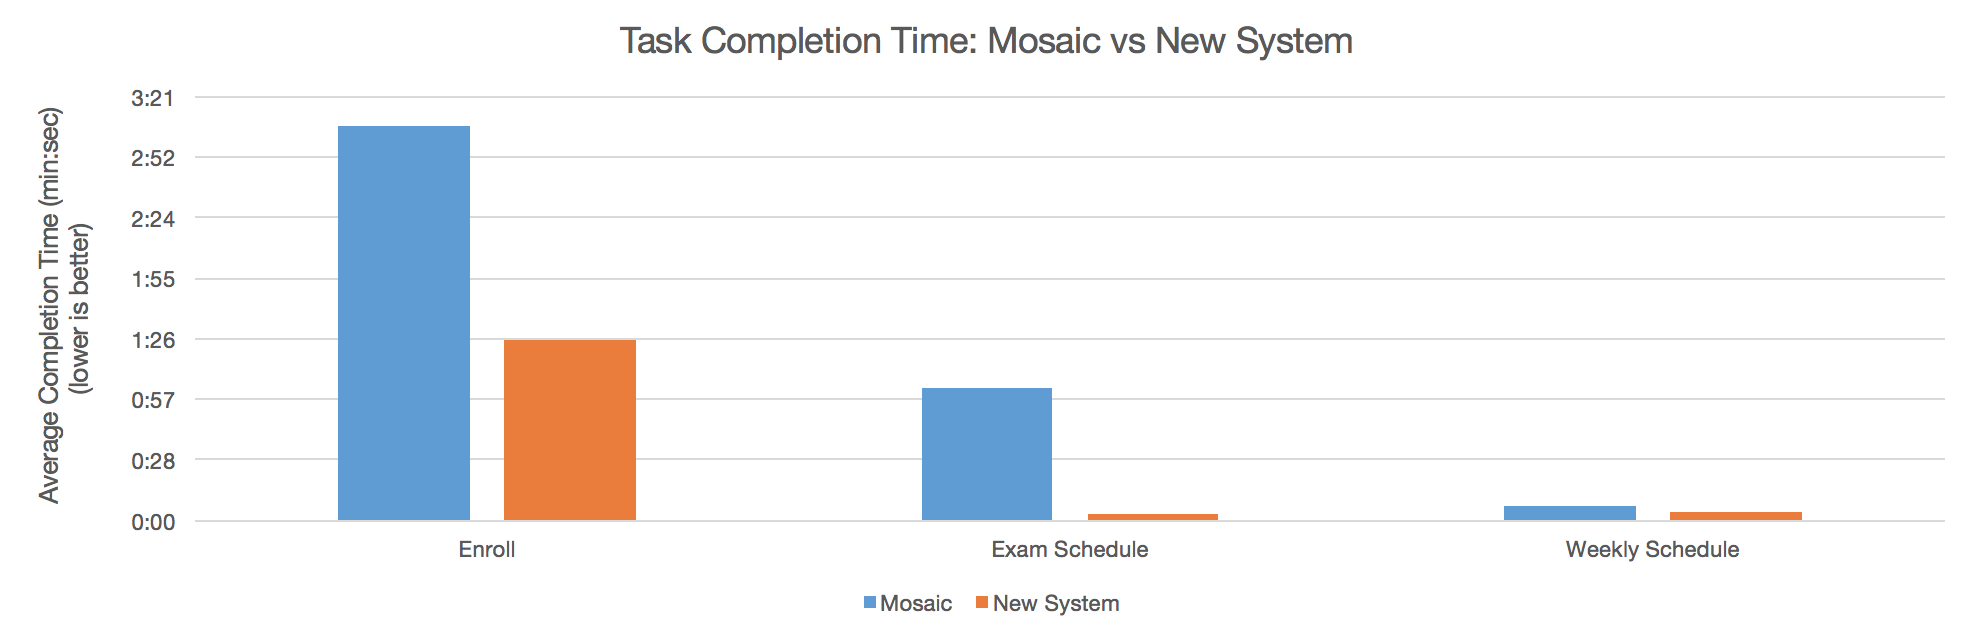
\includegraphics[width=0.7\textwidth]{images/results_avg_time.png}}\\
    \Caption{Task Completion Time: Mosaic vs New System}
\end{figure}

\begin{figure}[h]
    \centering
    \fbox{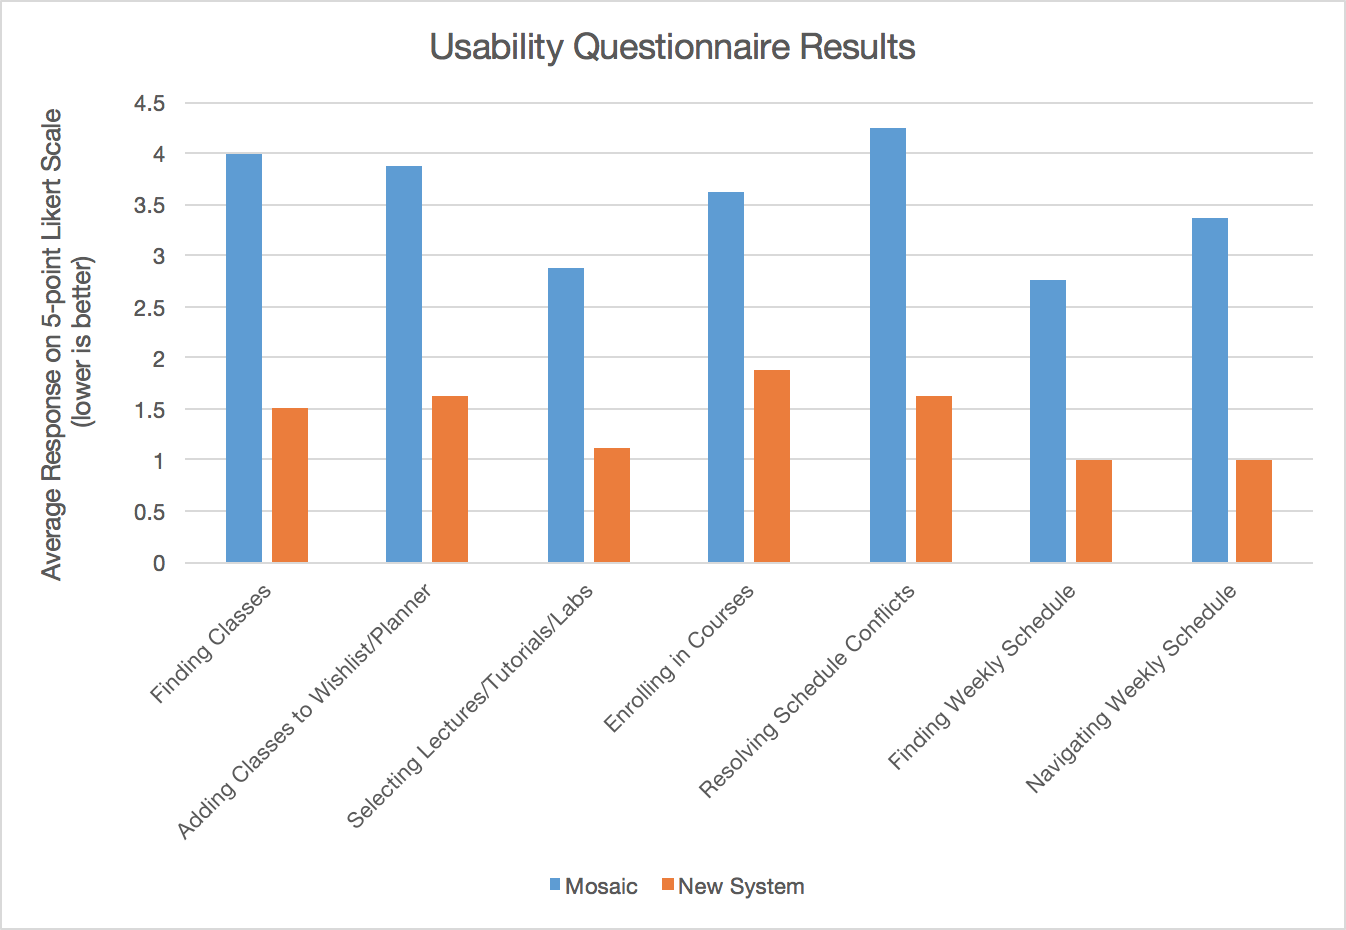
\includegraphics[width=0.7\textwidth]{images/results_avg_questionnaire.png}}\\
    \Caption{Usability Questionnaire Results}
\end{figure}

\begin{figure}[h]
    \centering
    \fbox{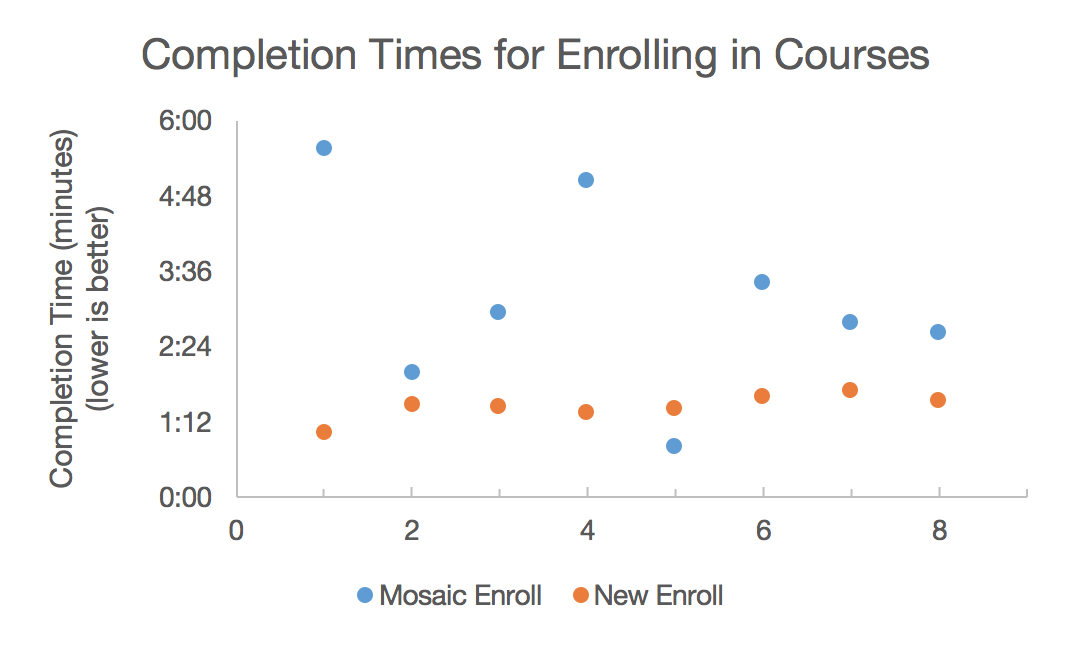
\includegraphics[width=0.7\textwidth]{images/results_enroll_time.png}}\\
    \Caption{Completion Times for Enrolling in Courses}
\end{figure}

\clearpage
\newpage
% ================== SUBSECTION ============================ %
\subsection*{Other Systems -- HTA's}
\begin{figure}[h]
    \centering
    \fbox{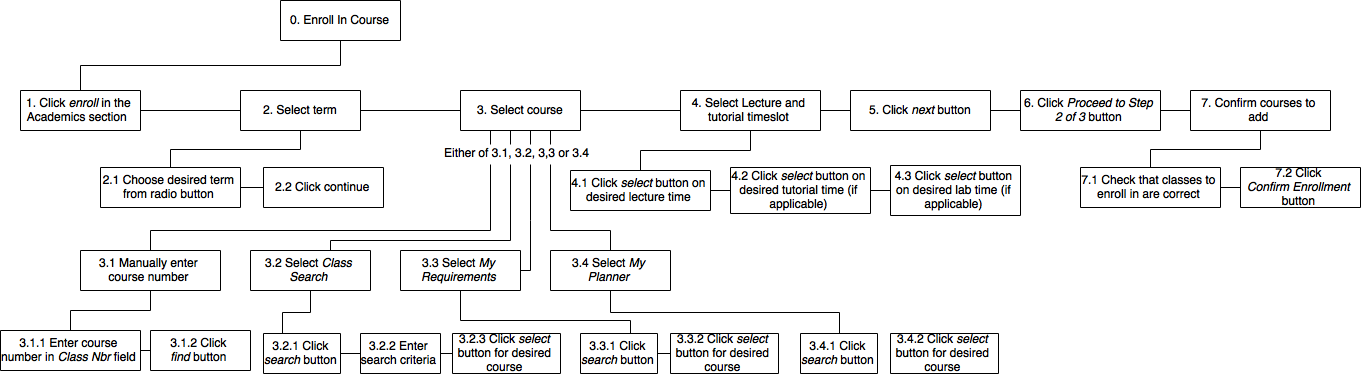
\includegraphics[width=\textwidth]{images/MosaicEnroll.png}}\\
    \Caption{Mosaic HTA -- Enrolling in a Course}
\end{figure}

\begin{figure}[h]
    \centering
    \fbox{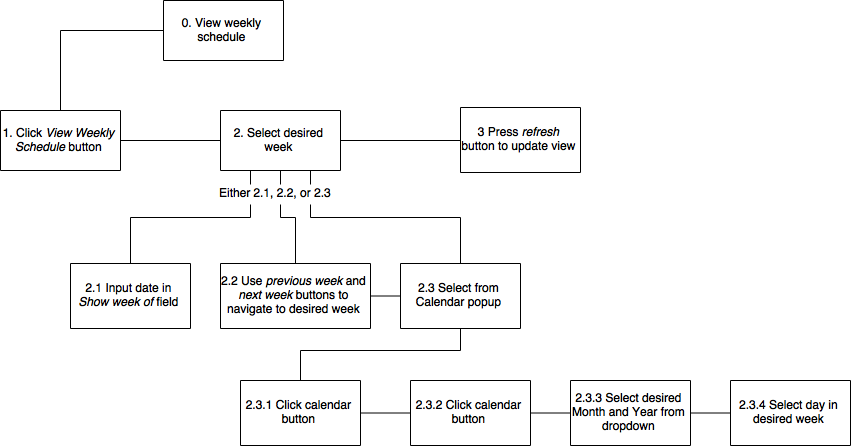
\includegraphics[width=\textwidth]{images/MosaicViewSchedule.png}}\\
    \Caption{Mosaic HTA -- Viewing Weekly Schedule}
\end{figure}

\begin{figure}[h]
    \centering
    \fbox{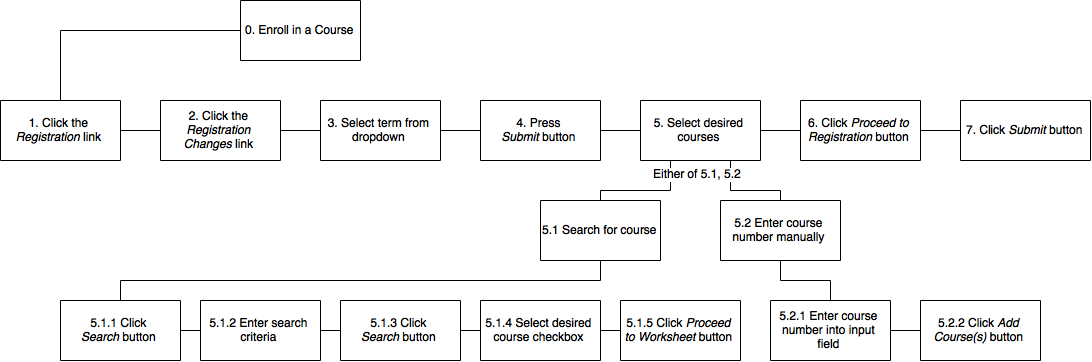
\includegraphics[width=\textwidth]{images/CarletonEnroll.png}}\\
    \Caption{Carleton HTA -- Enrolling in a Course}
\end{figure}

\begin{figure}[h]
    \centering
    \fbox{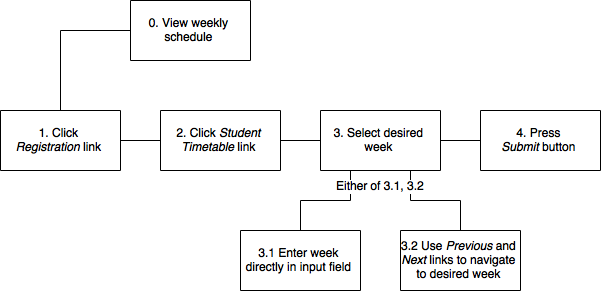
\includegraphics[width=0.6\textwidth]{images/CarletonViewSchedule.png}}\\
    \Caption{Carleton HTA -- Viewing Weekly Schedule}
\end{figure}

\begin{figure}[h]
    \centering
    \fbox{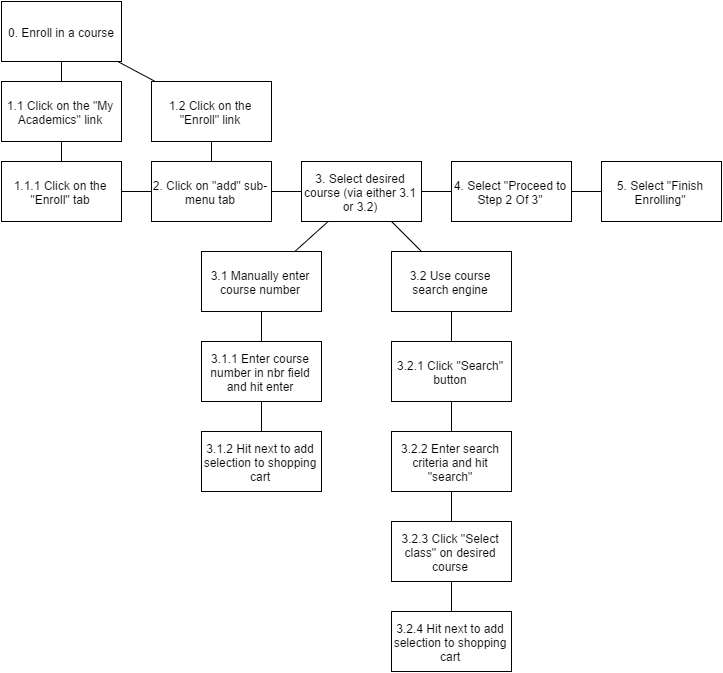
\includegraphics[width=0.6\textwidth]{images/WaterlooEnroll.png}}\\
    \Caption{Quest HTA -- Enrolling in a Course}
\end{figure}

\begin{figure}[h]
    \centering
    \fbox{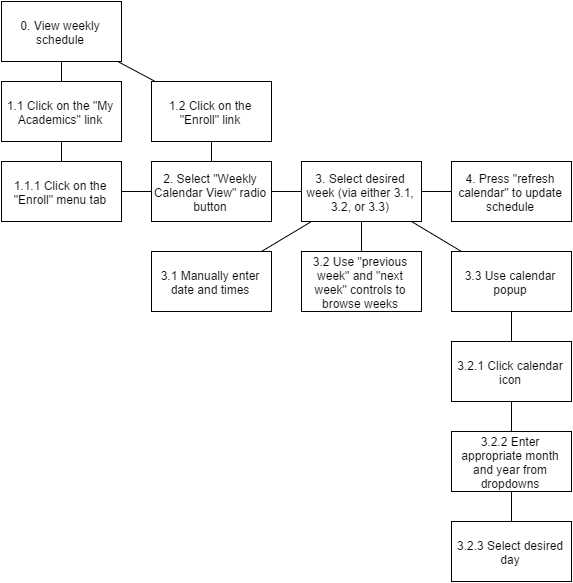
\includegraphics[width=0.6\textwidth]{images/WaterlooSchedule.png}}\\
    \Caption{Quest HTA -- Viewing Weekly Schedule}
\end{figure}

\begin{figure}[h]
    \centering
    \fbox{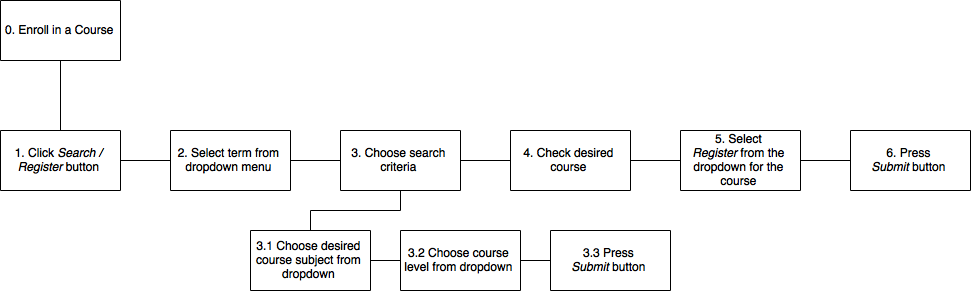
\includegraphics[width=\textwidth]{images/WebAdvisorEnroll.png}}\\
    \Caption{WebAdvisor HTA -- Enrolling in a Course}
\end{figure}

\begin{figure}[h]
    \centering
    \fbox{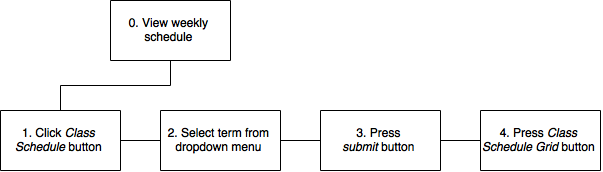
\includegraphics[width=\textwidth]{images/WebAdvisorViewSchedule.png}}\\
    \Caption{WebAdvisor HTA -- Viewing Weekly Schedule}
\end{figure}

% ================== SUBSECTION ============================ %
\clearpage
\subsection*{Other Systems -- Screenshots}

\begin{minipage}{.5\textwidth}
    \centering
    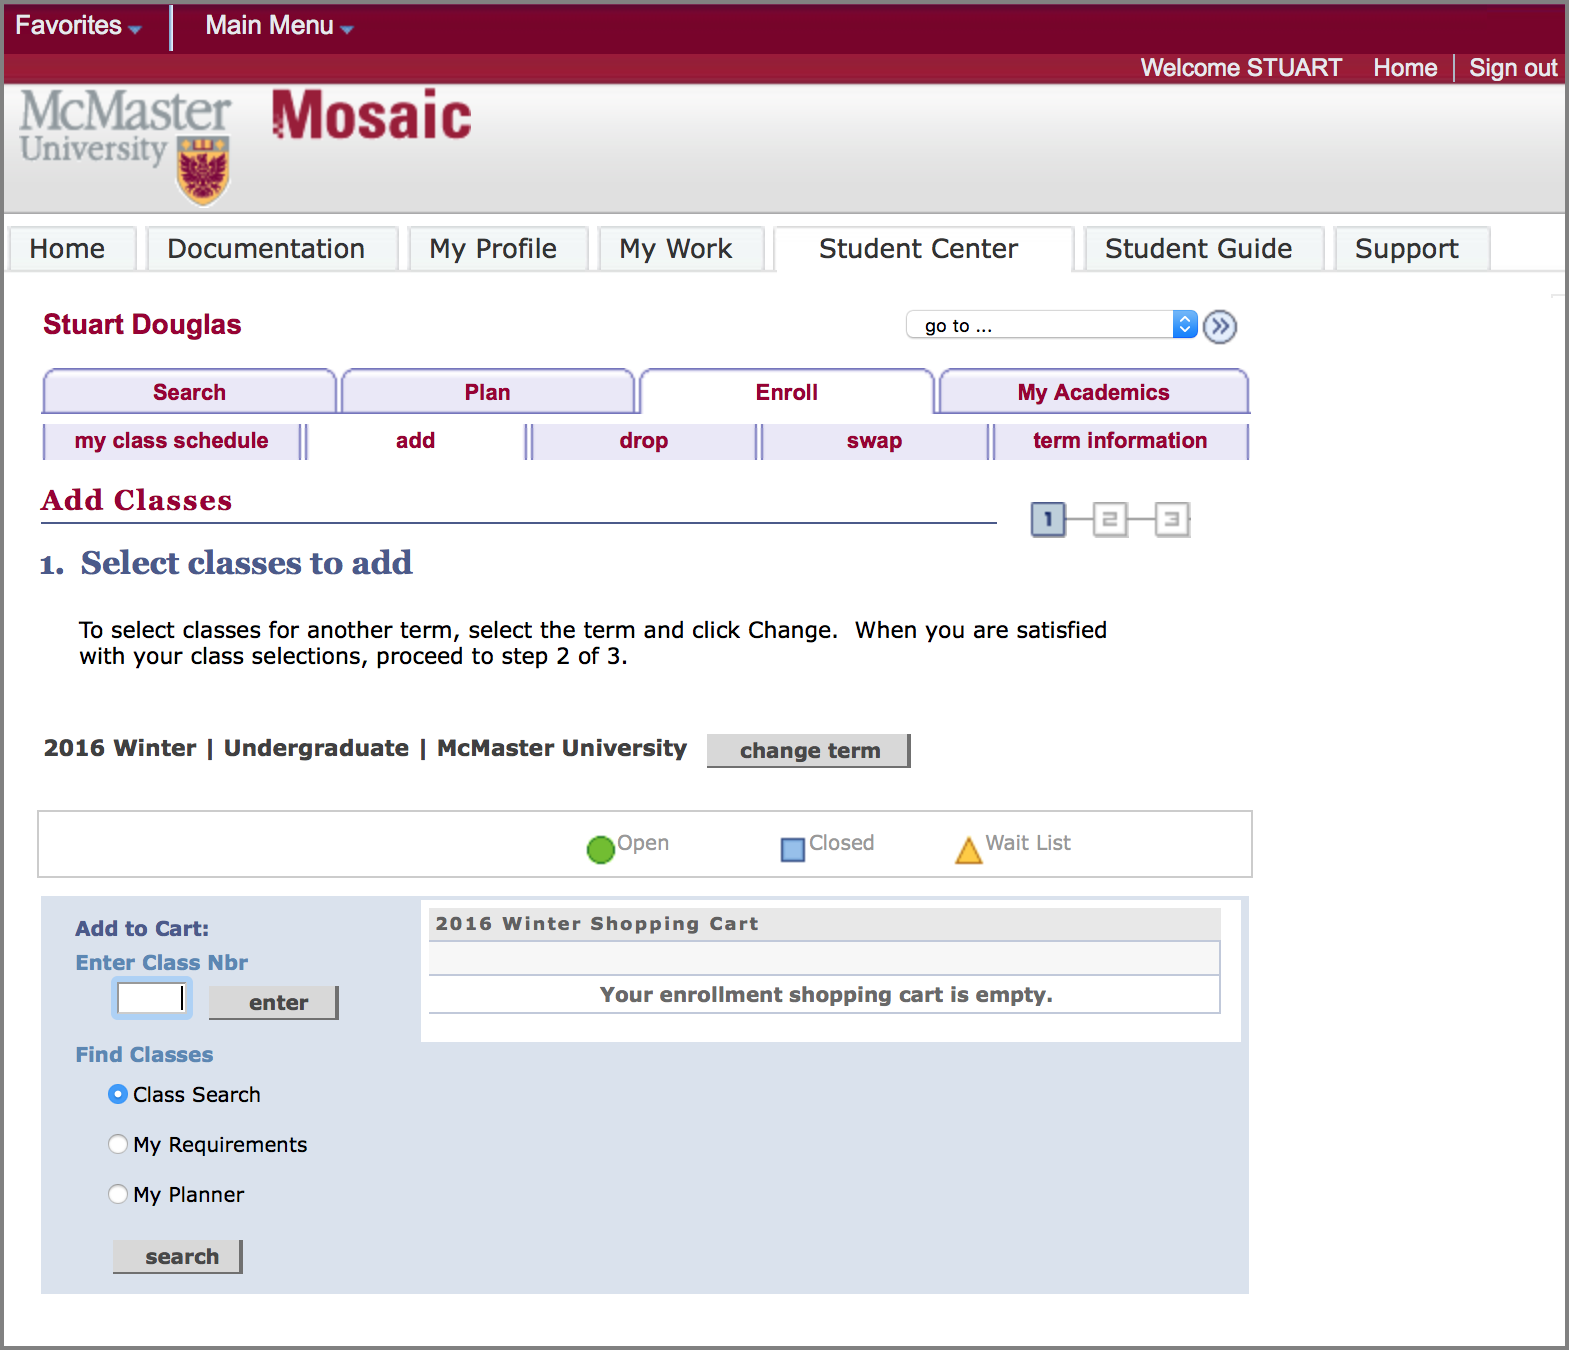
\includegraphics[height=70mm]{images/MosaicScreen.png}\\
    \Caption{Mosaic -- Screenshot}
\end{minipage}
\begin{minipage}{.5\textwidth}
    \centering
    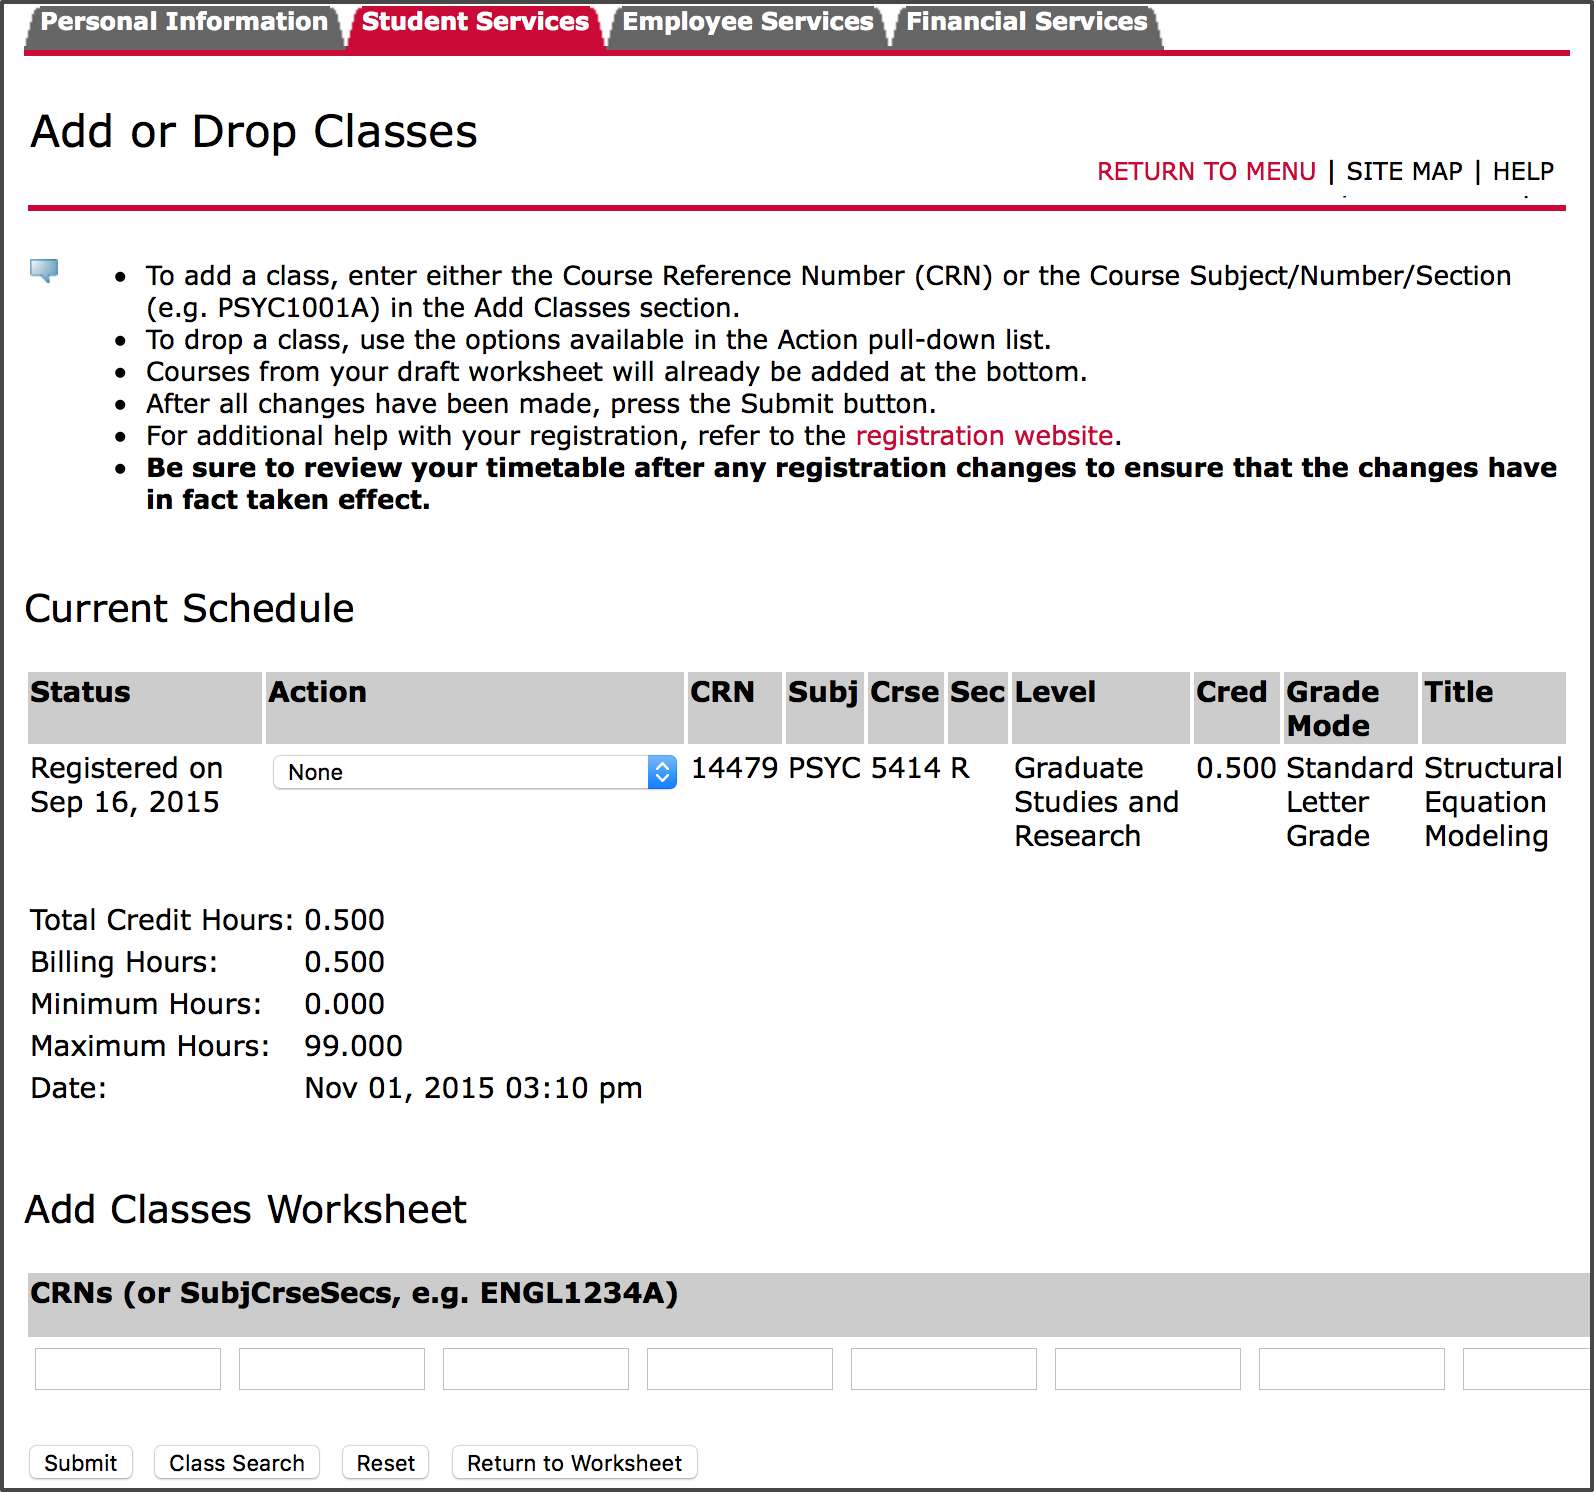
\includegraphics[height=70mm]{images/CarletonScreen.png}\\
    \Caption{Carleton -- Screenshot}
\end{minipage}\\\vspace{5mm}

\begin{minipage}{.5\textwidth}
    \centering
    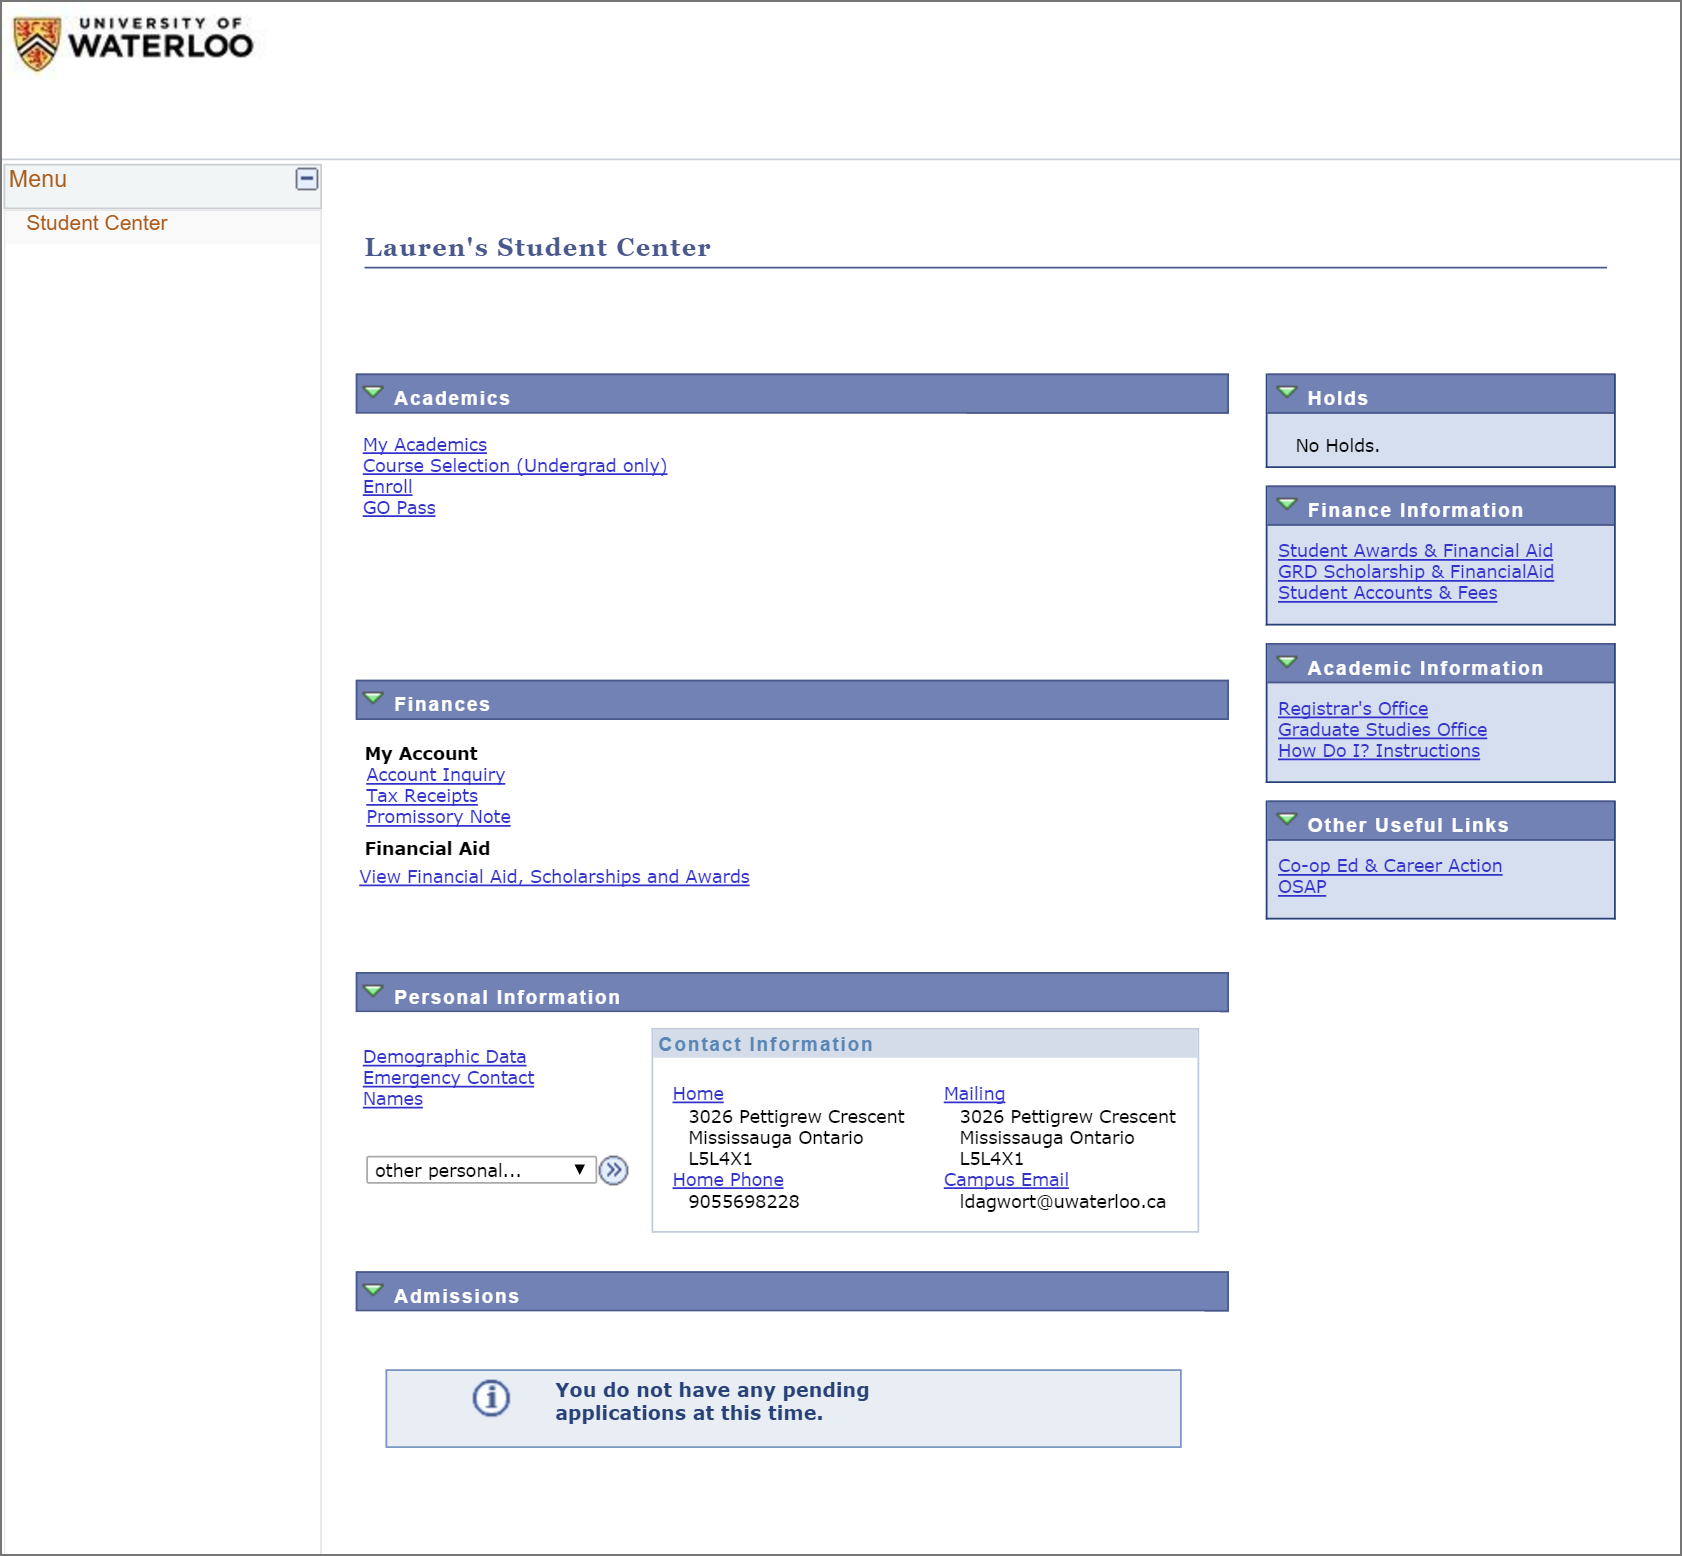
\includegraphics[height=70mm]{images/WaterlooScreen.png}\\
\Caption{Quest -- Screenshot}
\end{minipage}
\begin{minipage}{.5\textwidth}
    \centering
	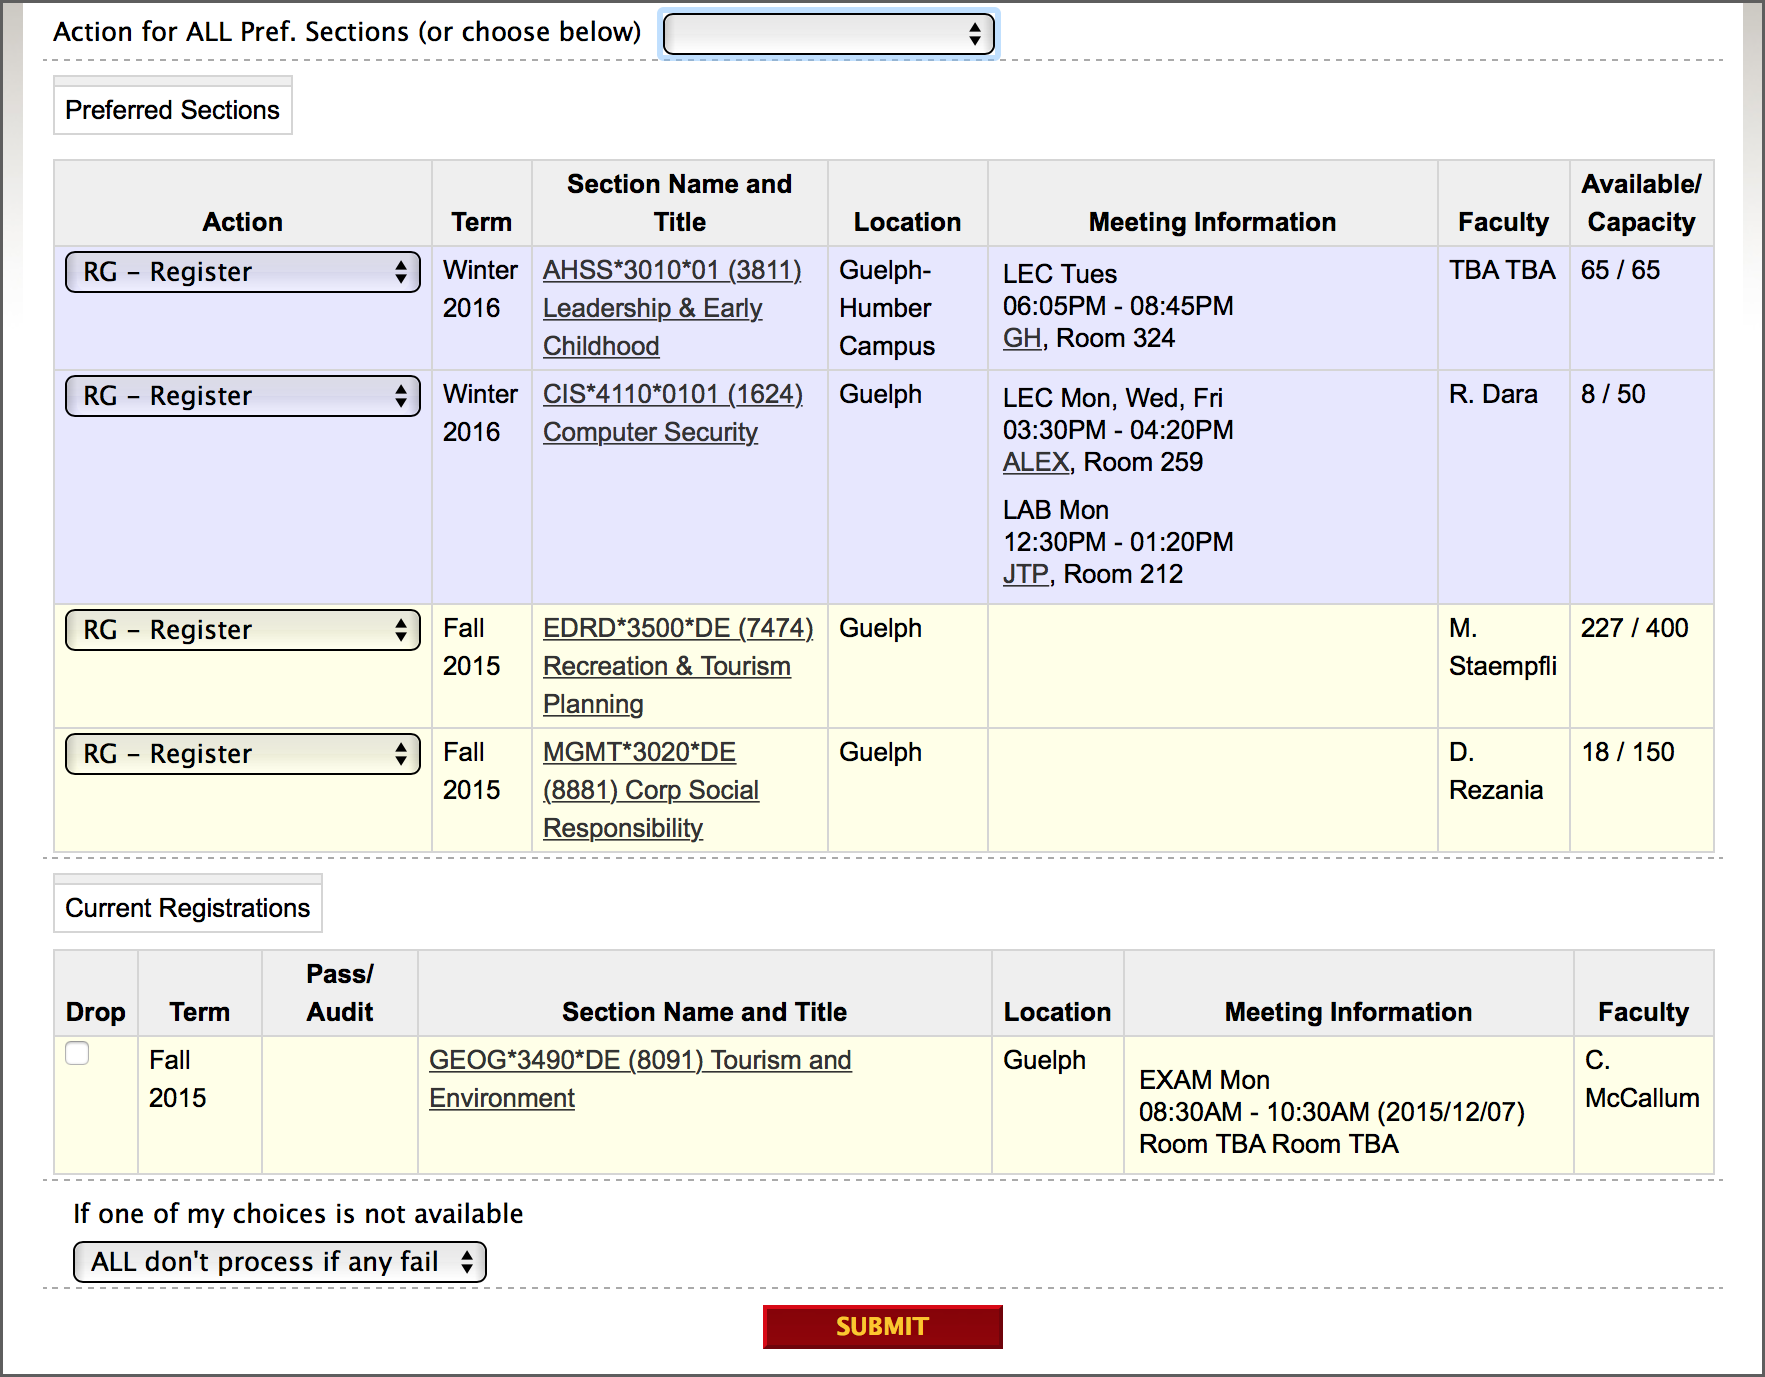
\includegraphics[height=70mm]{images/WebAdvisorScreen.png}\\
	\Caption{WebAdvisor -- Screenshot}
\end{minipage}\\\vspace{3mm}

% ================== SUBSECTION ============================ %
\subsection*{New System -- Final Design Mockups}
\begin{minipage}{.5\textwidth}
    \centering
    \fbox{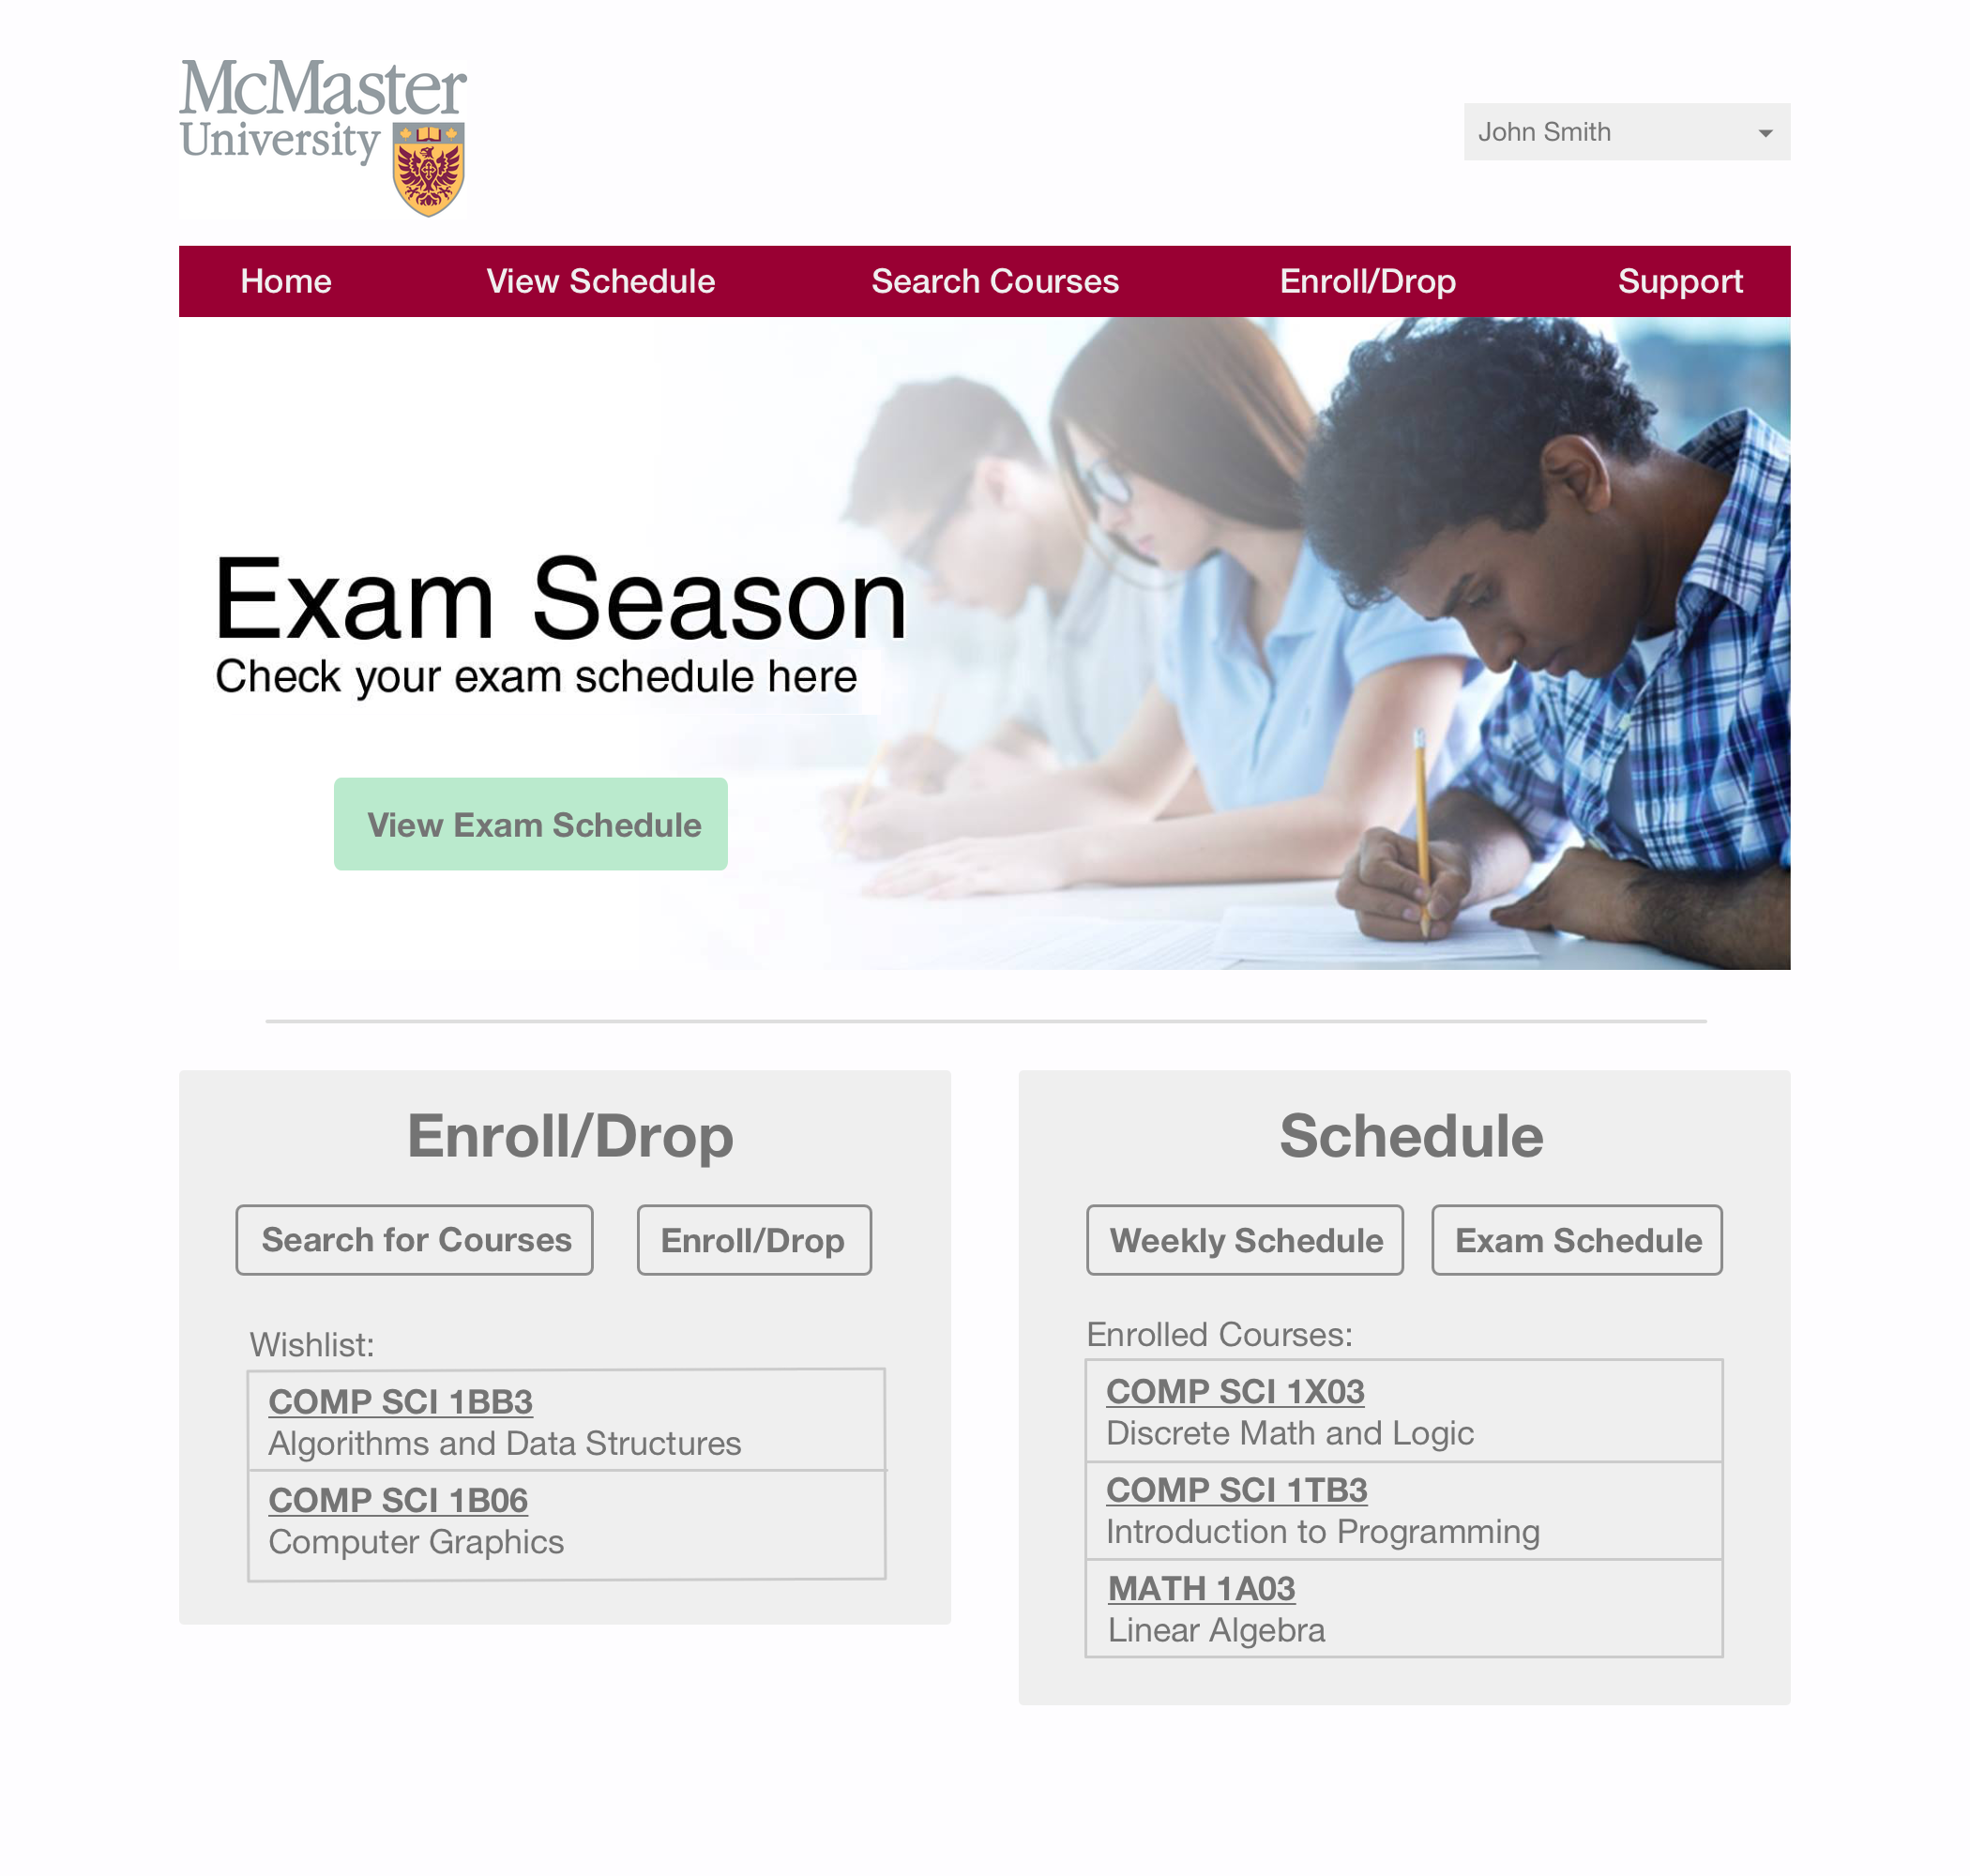
\includegraphics[height=80mm]{images/Rev2_MainPage.png}}\\
    \Caption{Final Mockup of Home Page}
\end{minipage}
\begin{minipage}{.5\textwidth}
    \centering
    \fbox{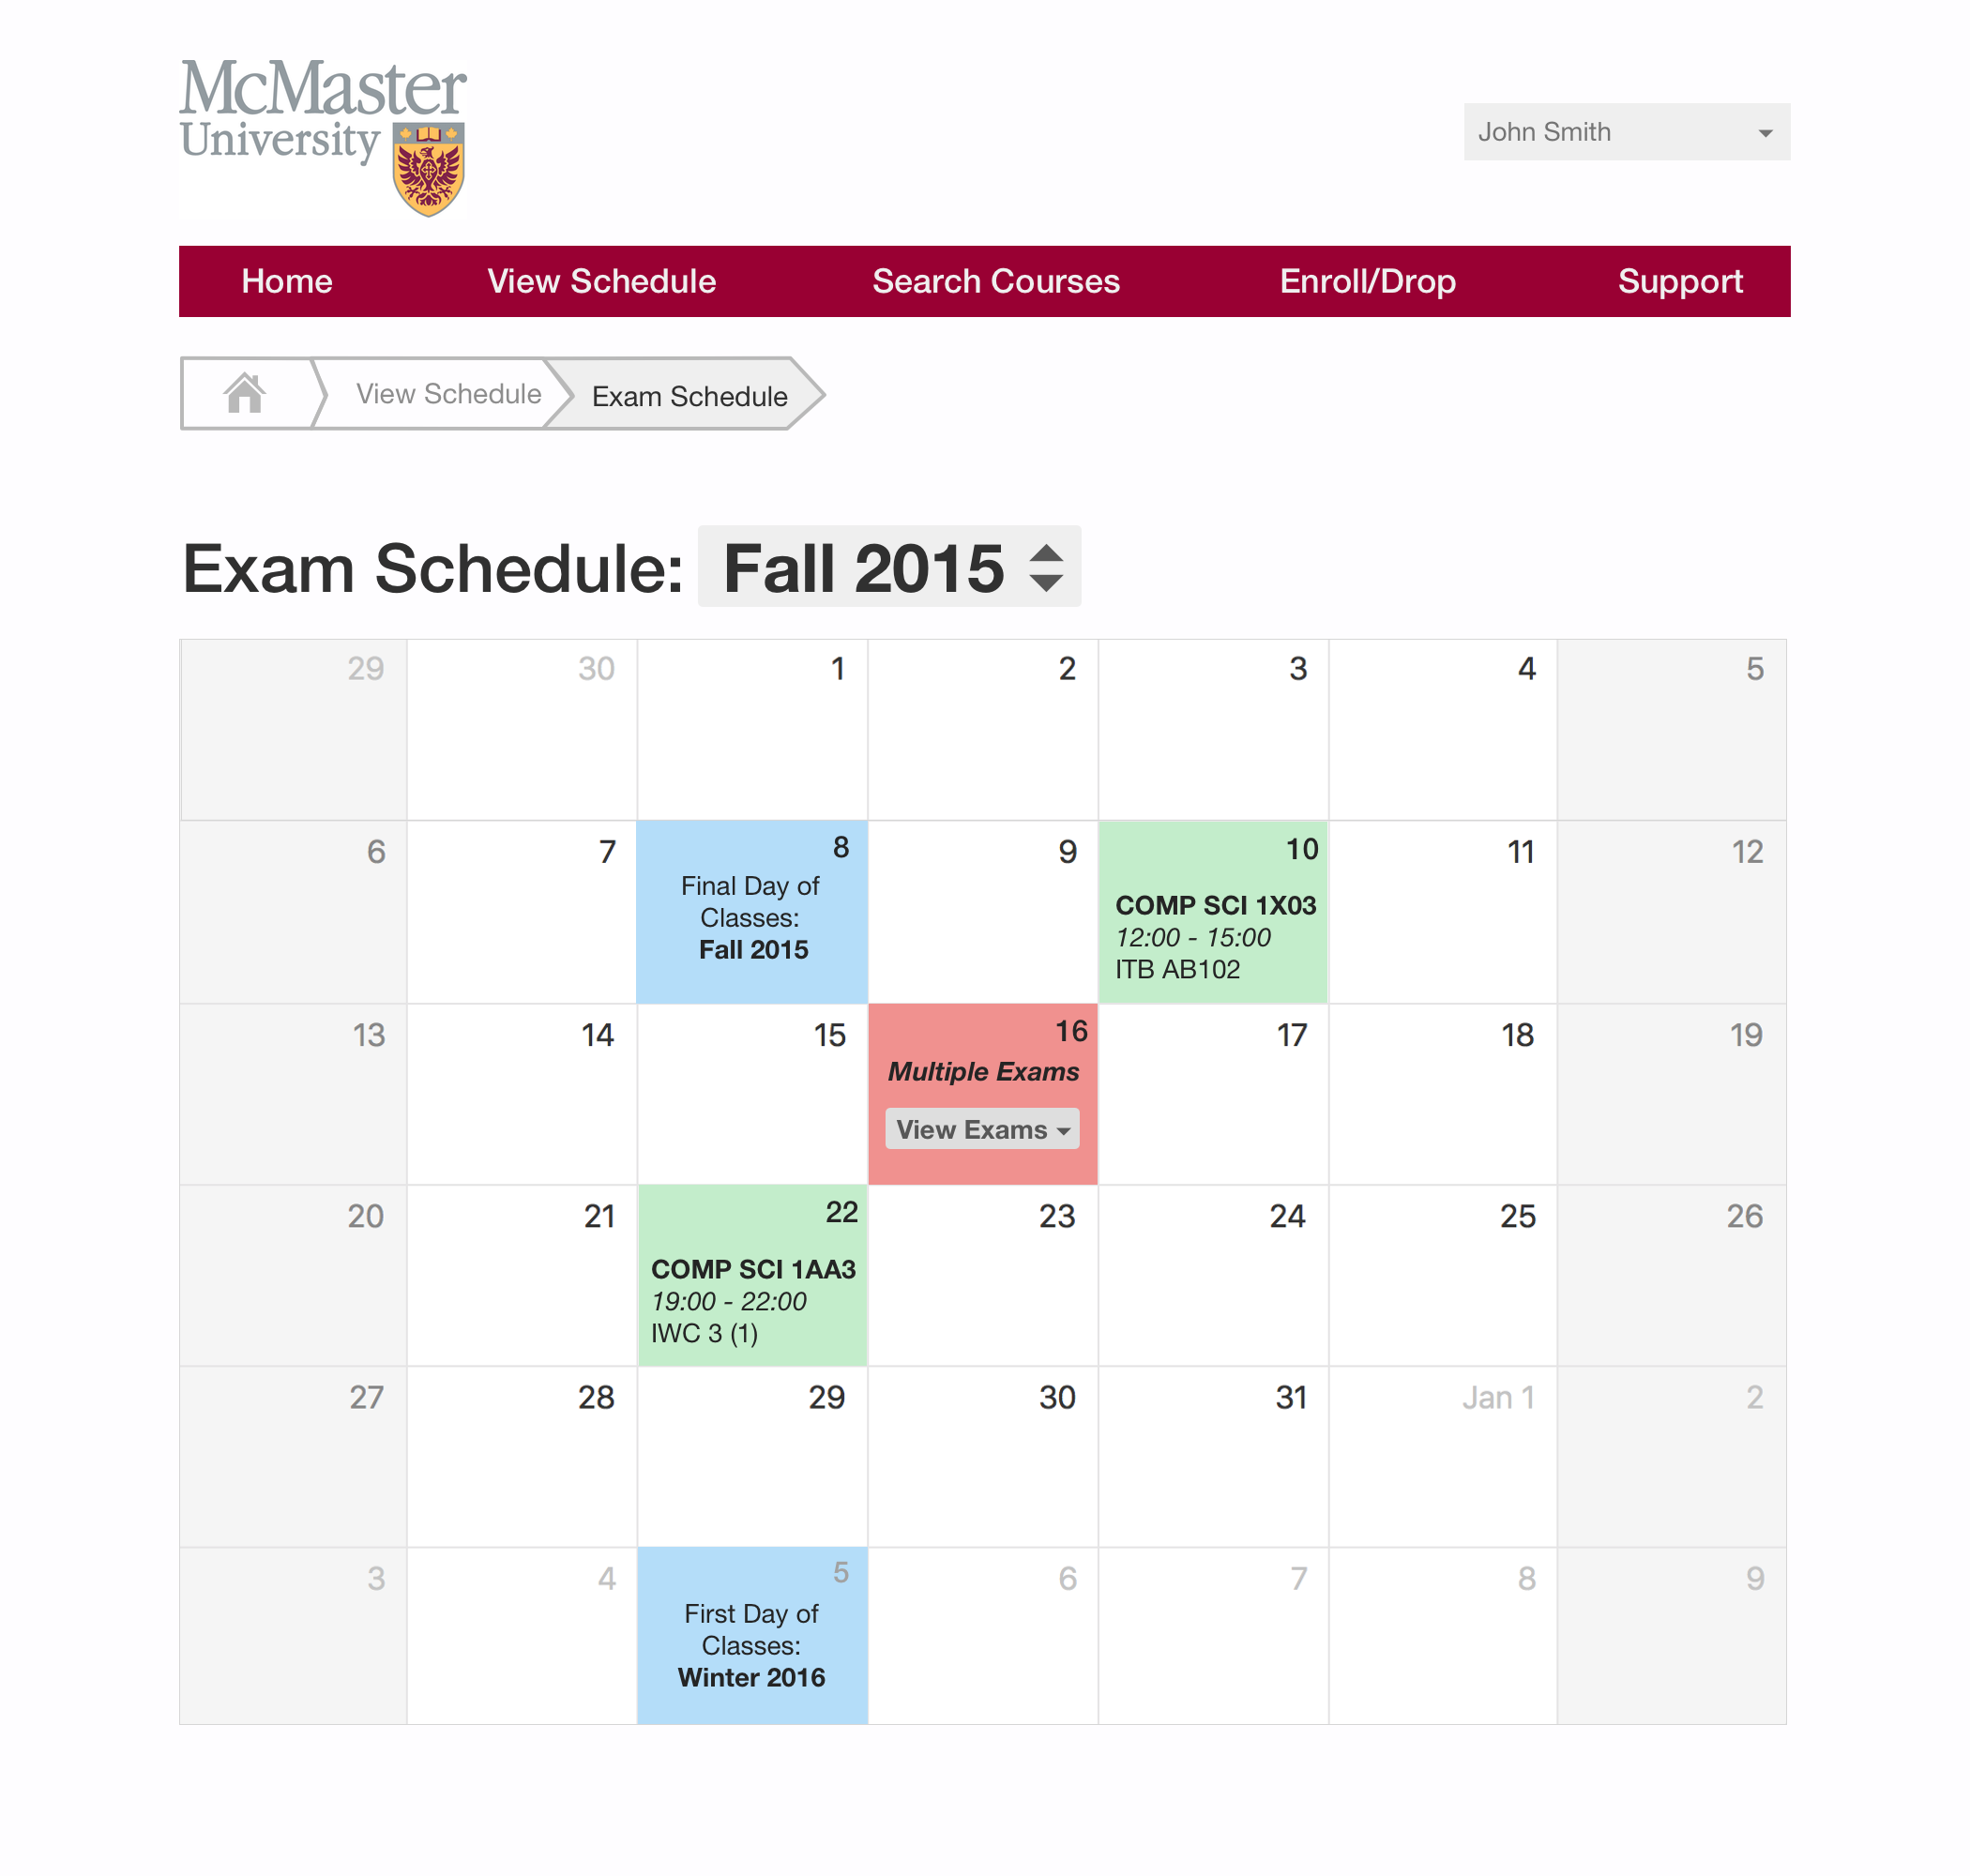
\includegraphics[height=80mm]{images/Rev2_ExamSchedule.png}}\\
    \Caption{Final Mockup of Exam Schedule}
\end{minipage}\\\vspace{5mm}

\begin{minipage}{.5\textwidth}
    \centering
    \fbox{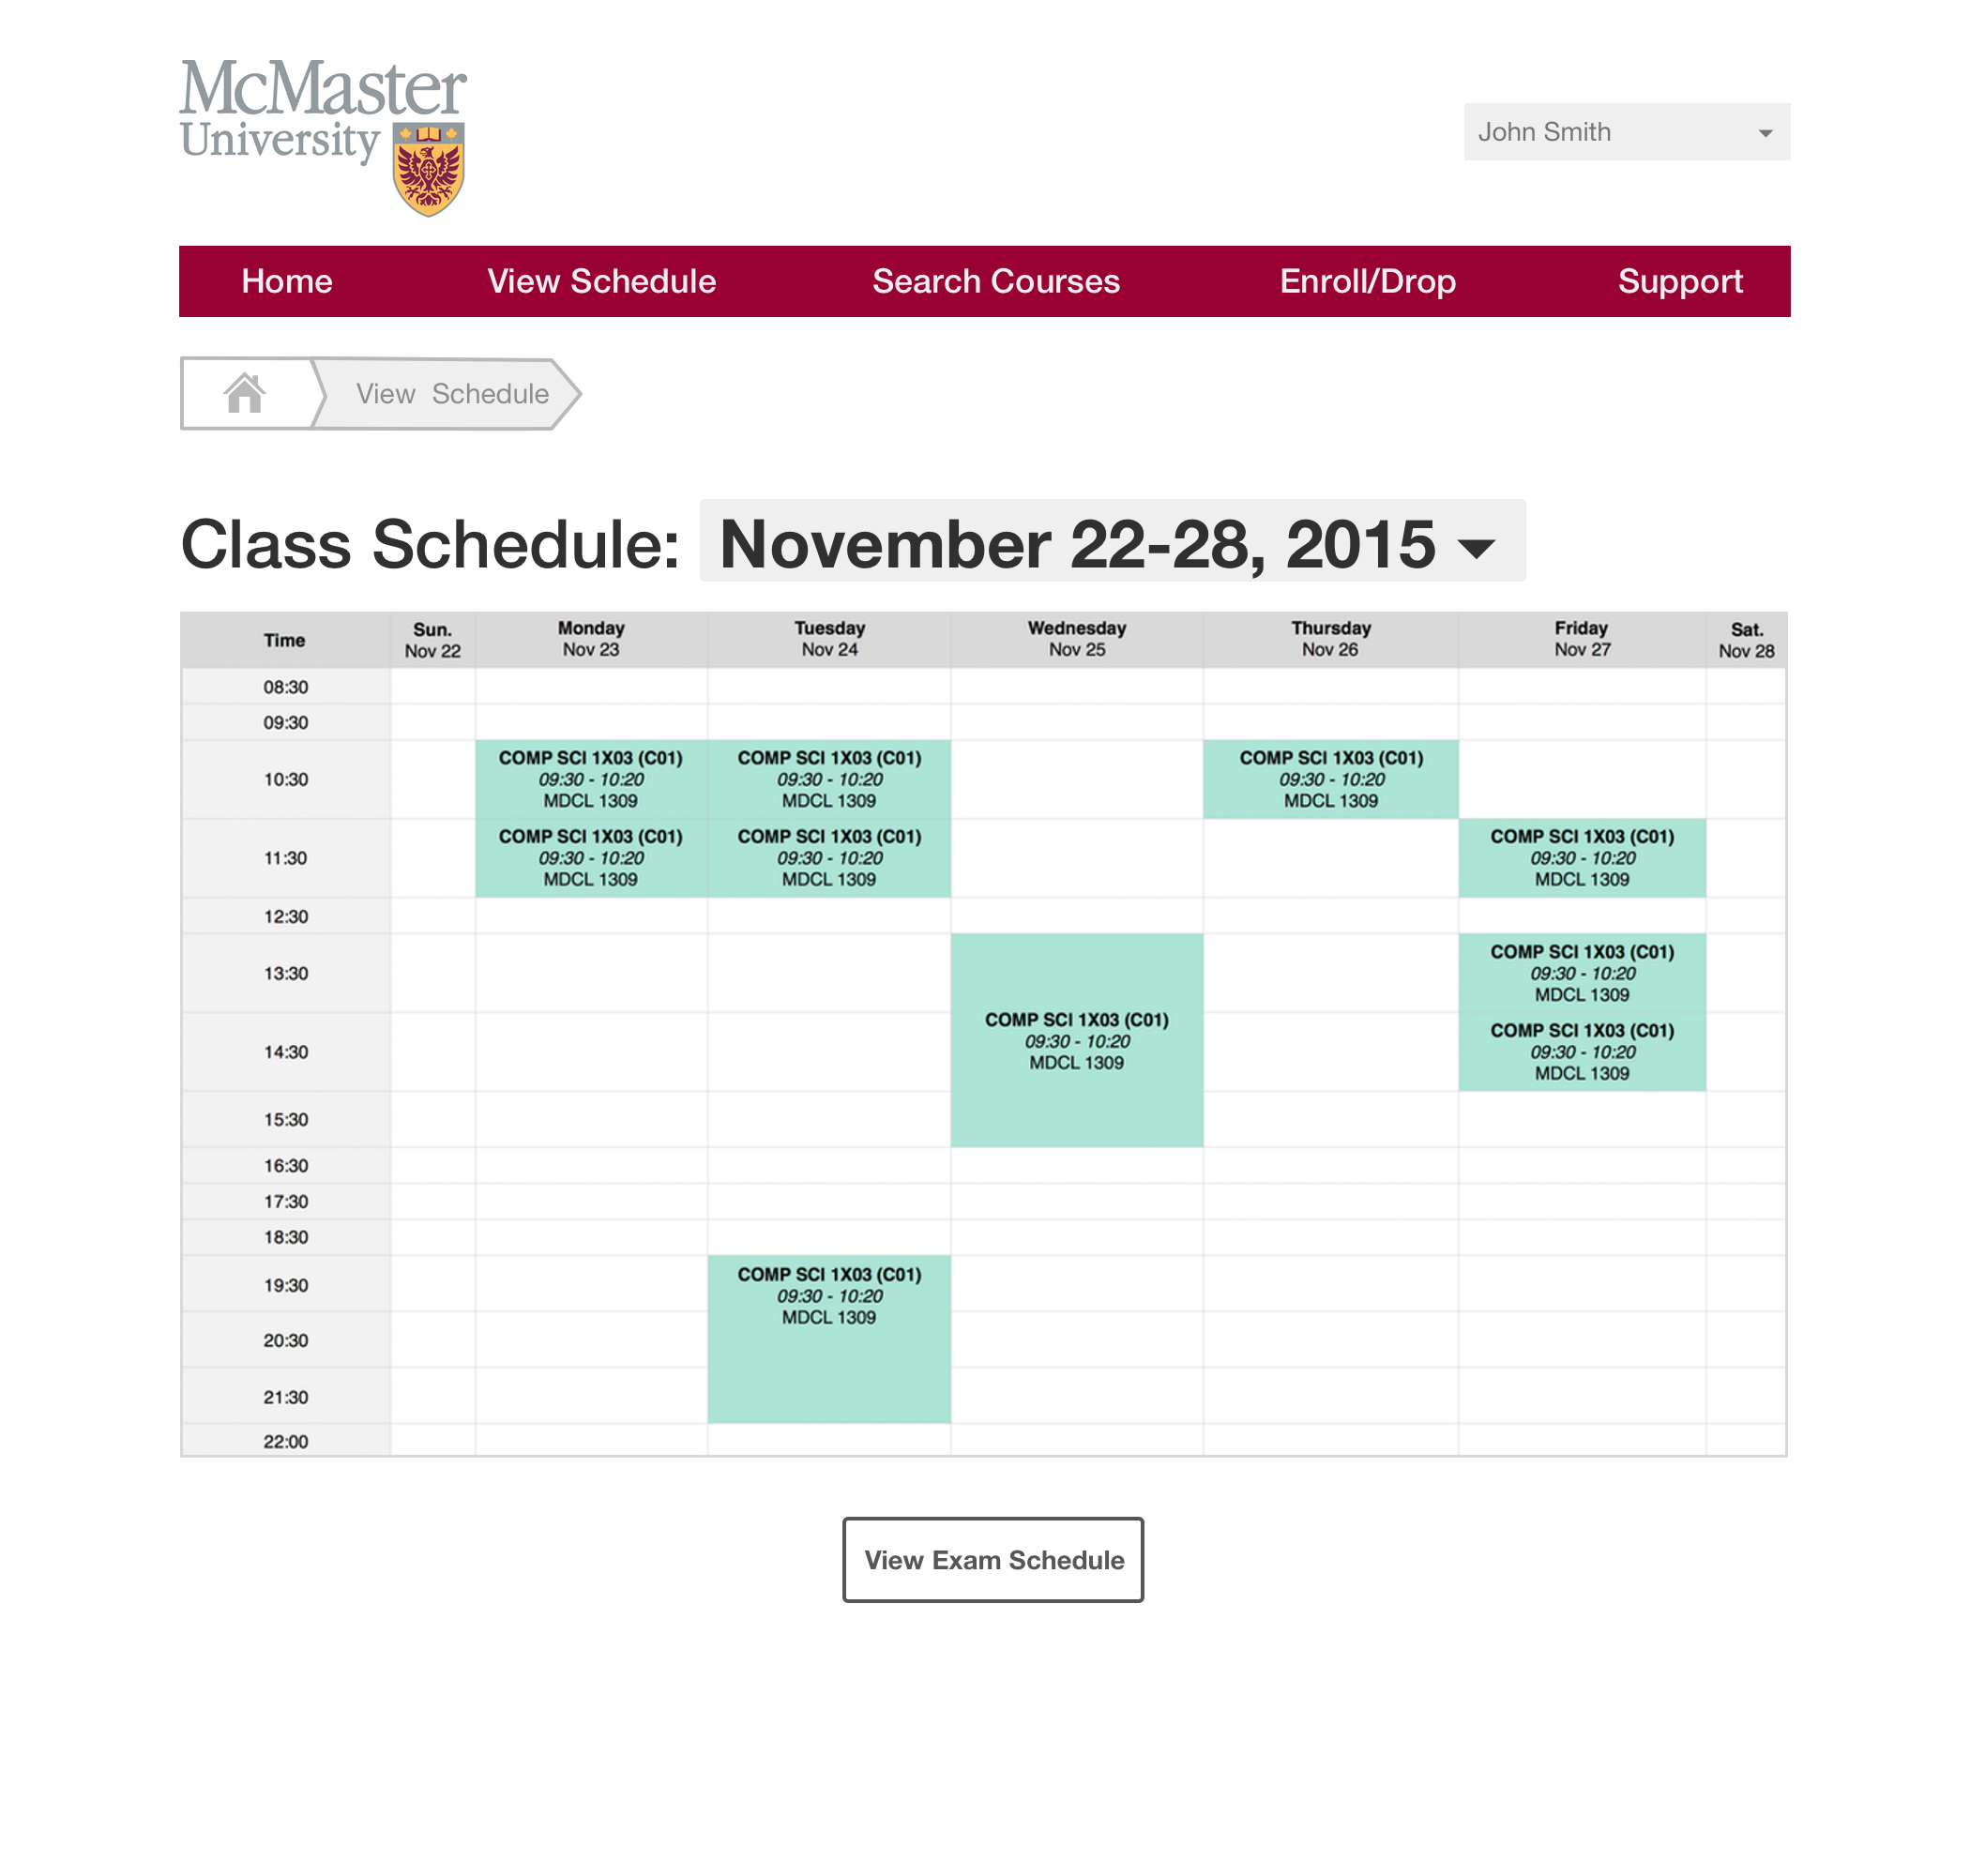
\includegraphics[height=80mm]{images/Rev2_WeeklySchedule.png}}\\
	\Caption{Final Mockup of Weekly Schedule}
\end{minipage}
\begin{minipage}{.5\textwidth}
    \centering
	\fbox{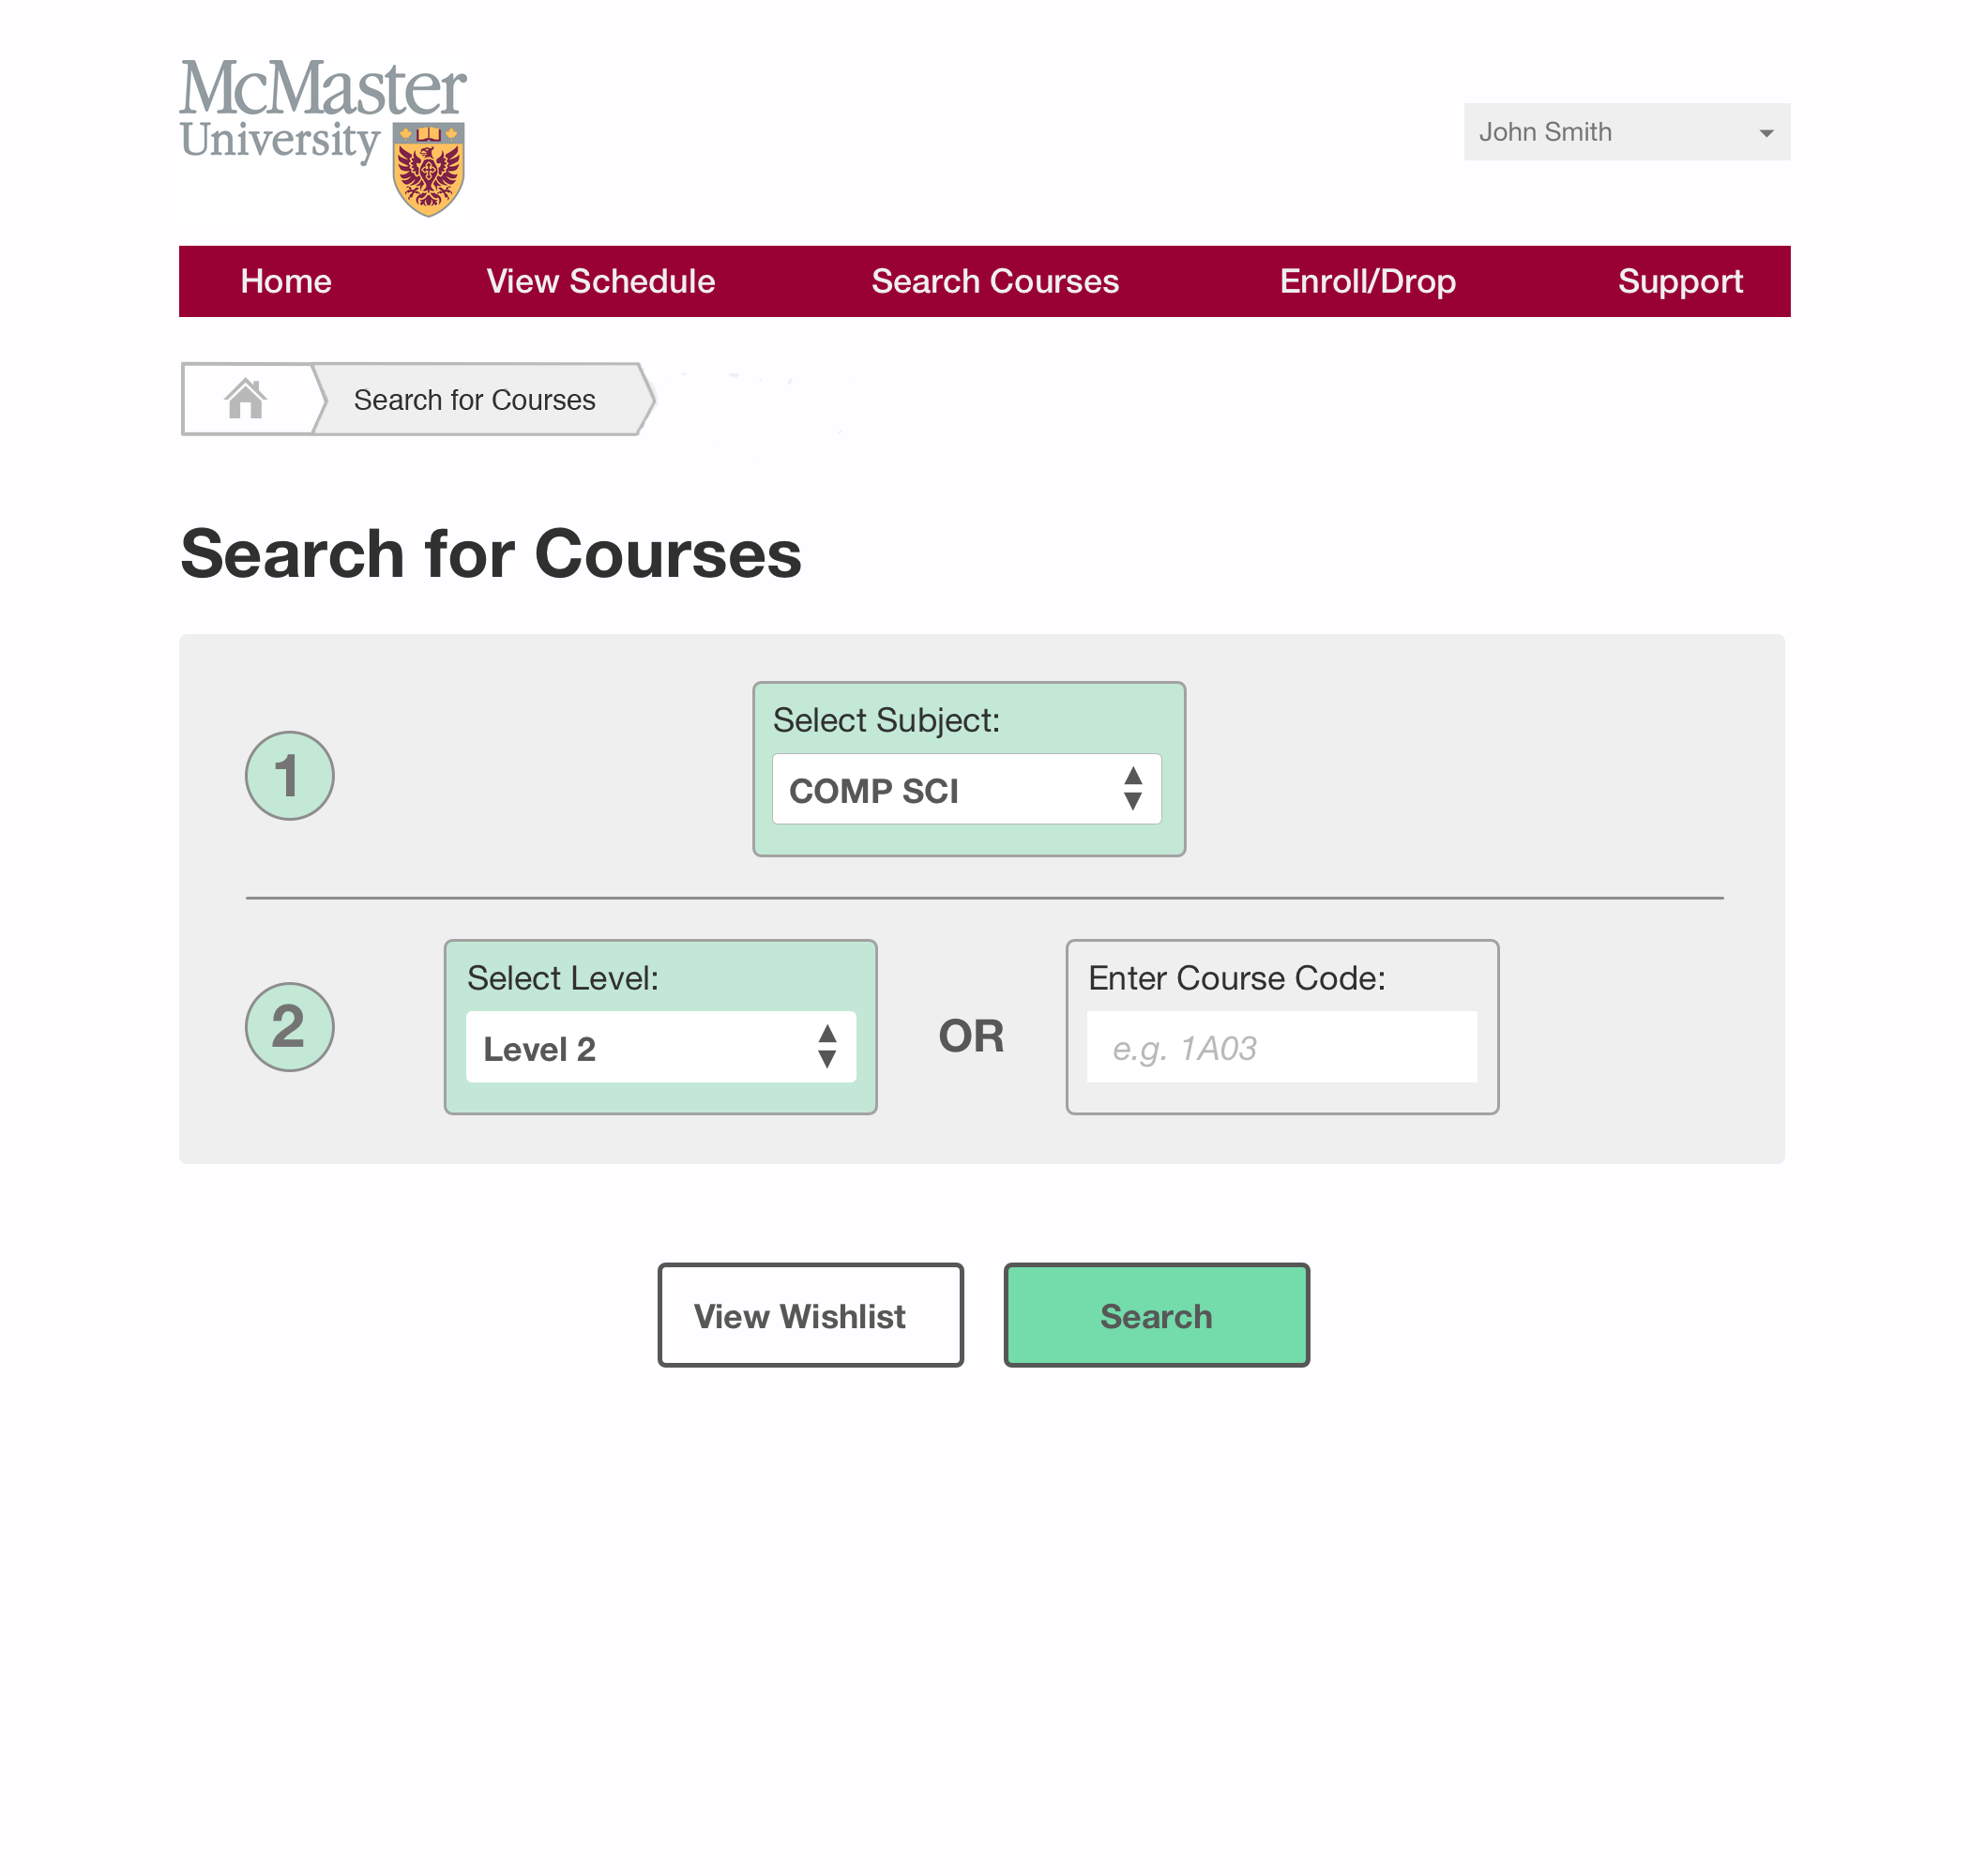
\includegraphics[height=80mm]{images/Rev2_SearchCourses.png}}\\
	\Caption{Final Mockup of Search Criteria Page}
\end{minipage}\\\vspace{3mm}

\begin{minipage}{.5\textwidth}
    \centering
    \fbox{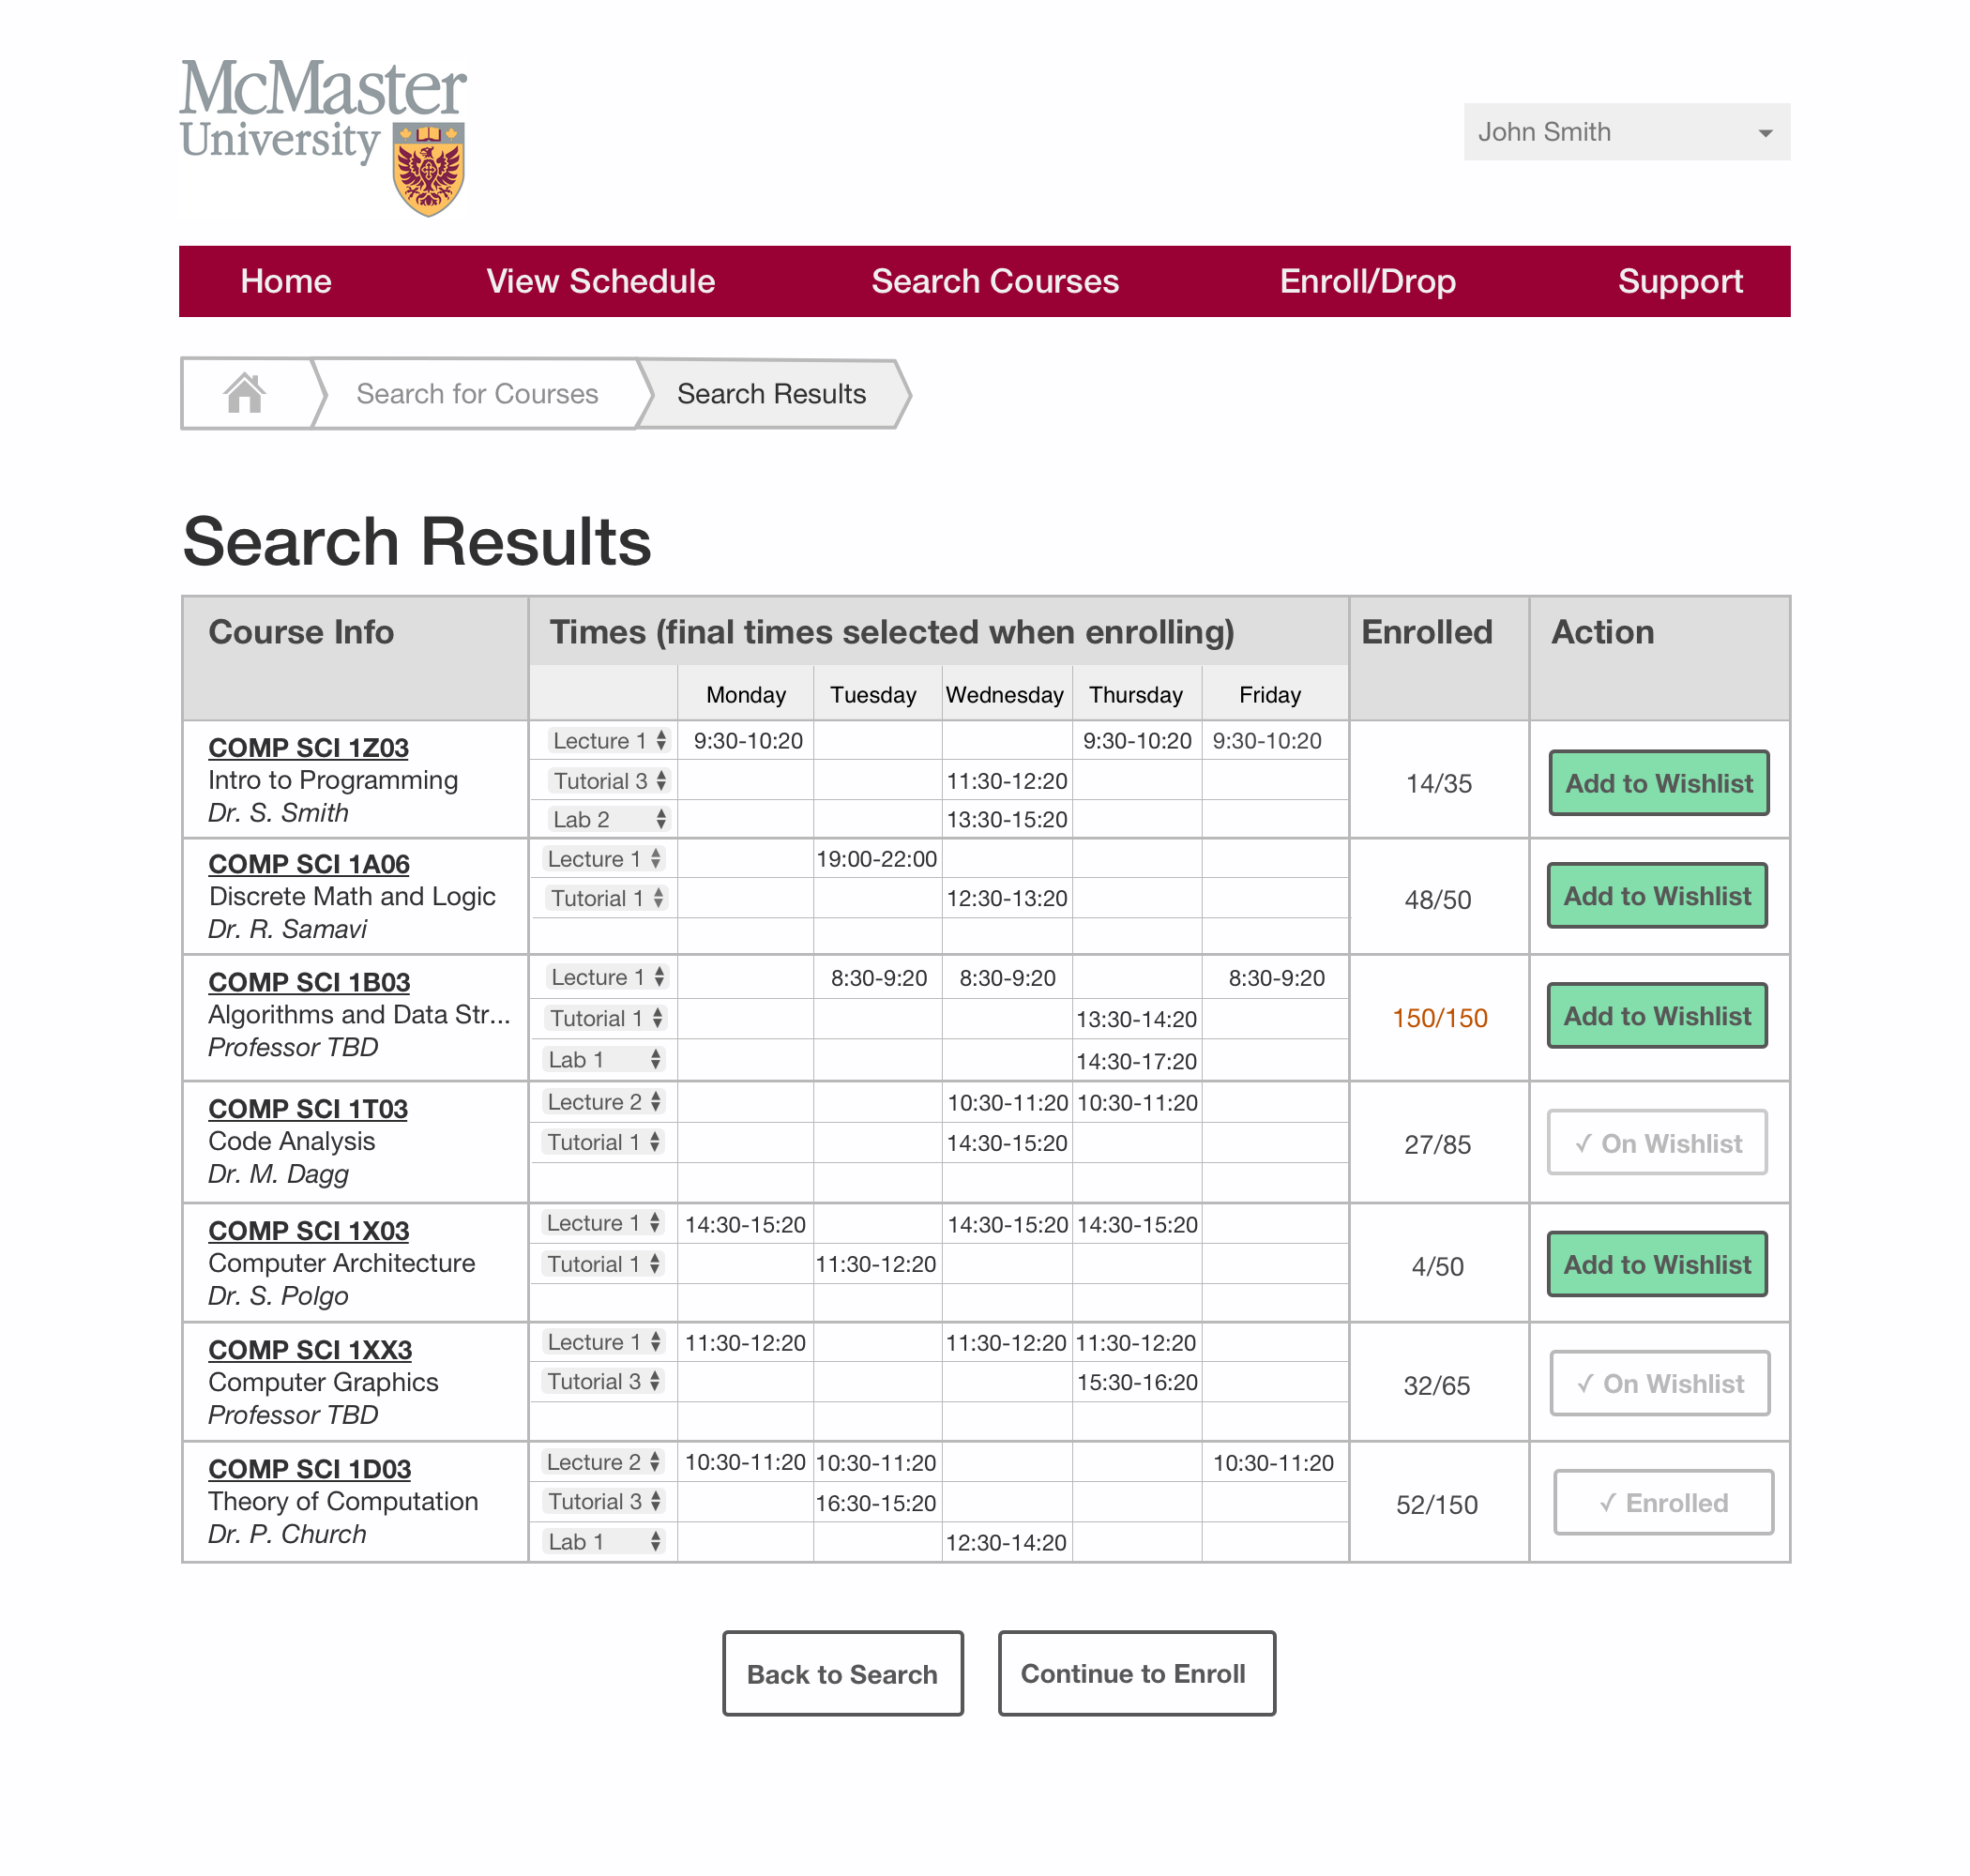
\includegraphics[height=80mm]{images/Rev2_CourseListing.png}}\\
    \Caption{Final Mockup of Search Results Page}
\end{minipage}
\begin{minipage}{.5\textwidth}
    \centering
    \fbox{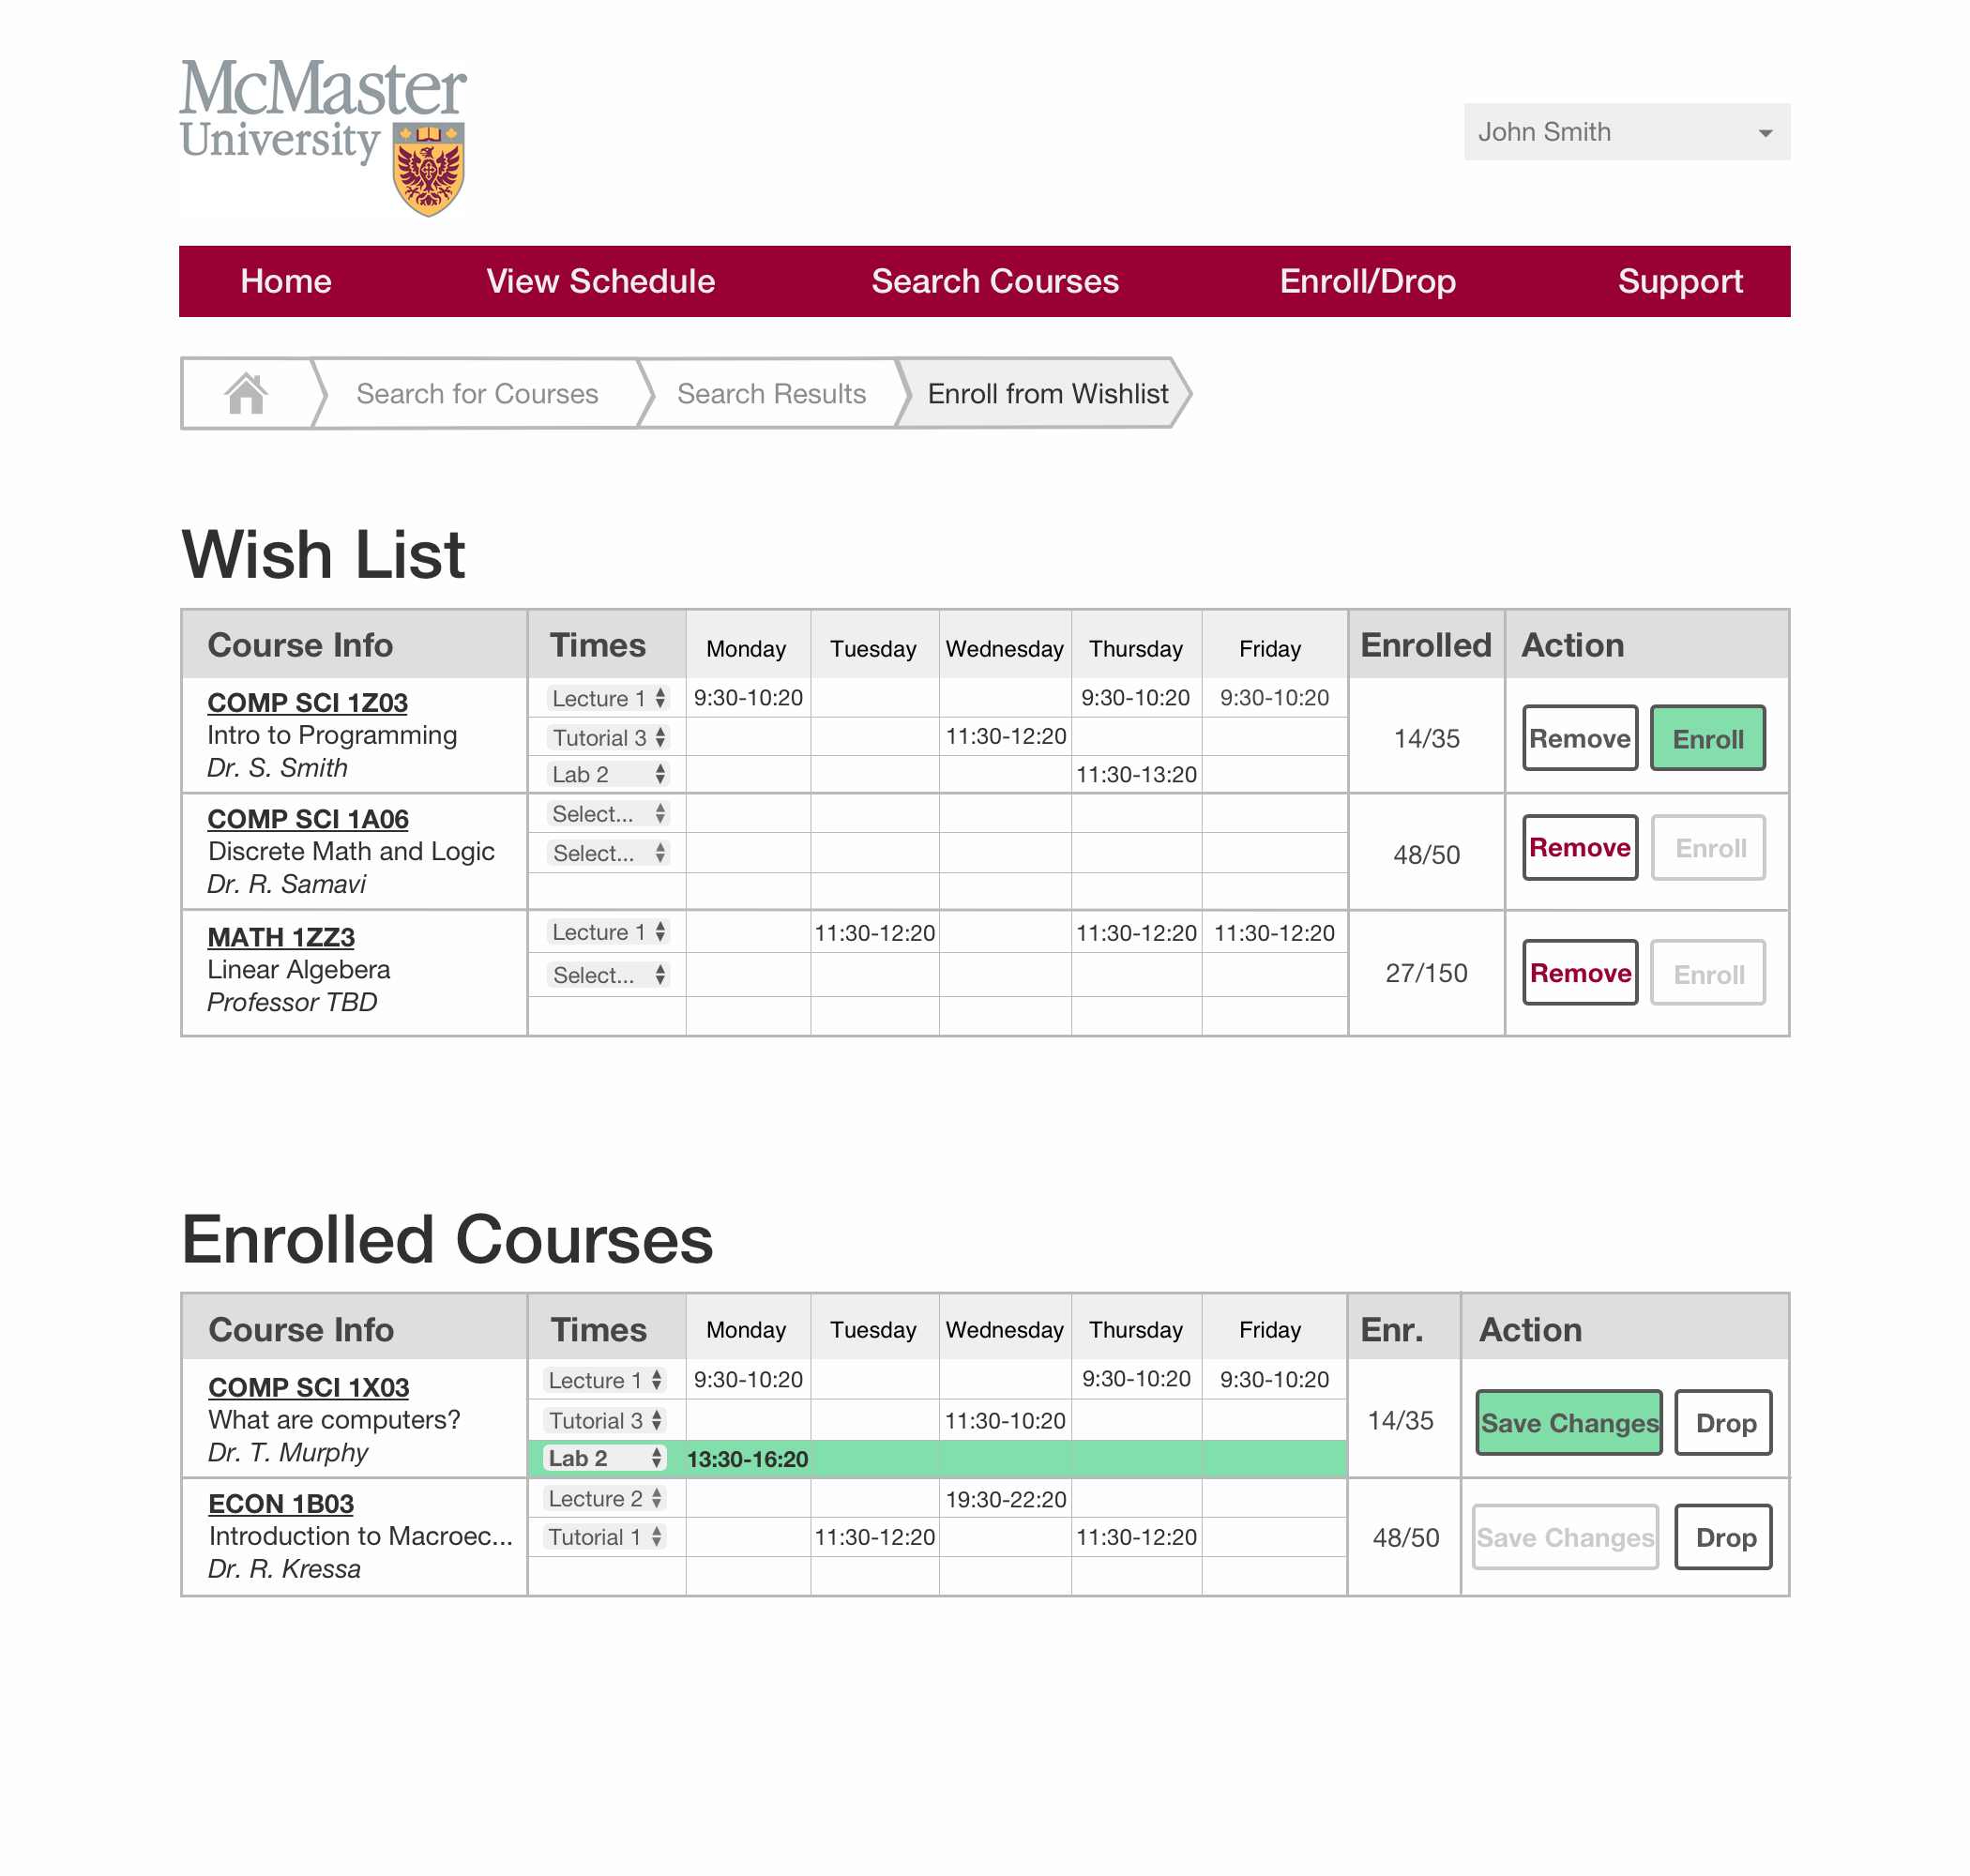
\includegraphics[height=80mm]{images/Rev2_WishlistEnroll.png}}\\
    \Caption{Final Mockup of Enroll from Wishlist Page}
\end{minipage}\\\vspace{5mm}

% ================== SUBSECTION ============================ %
\subsection*{New System -- HTA's}
\begin{figure}[h]
\centering
\fbox{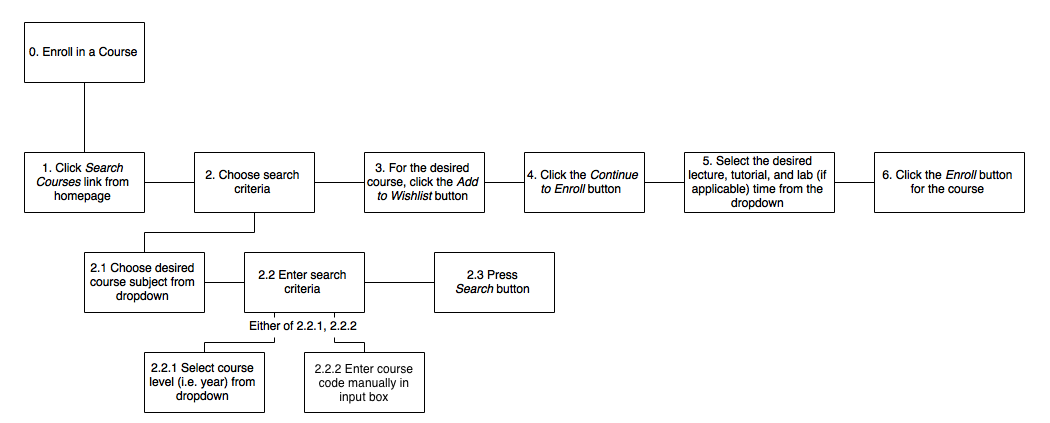
\includegraphics[width=\textwidth]{images/HTA_Enroll.png}}\\
\Caption{New System HTA - Enrolling in a Course}
\end{figure}

\begin{figure}[h]
\centering
\fbox{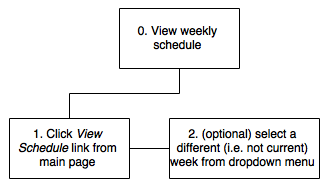
\includegraphics[width=60mm]{images/HTA_ViewSchedule.png}}\\
\Caption{New System HTA - View Weekly Schedule}
\end{figure}

% ================== SUBSECTION ============================ %
\subsection*{New System -- Screenshots}
\begin{figure}[h]
    \centering
    \fbox{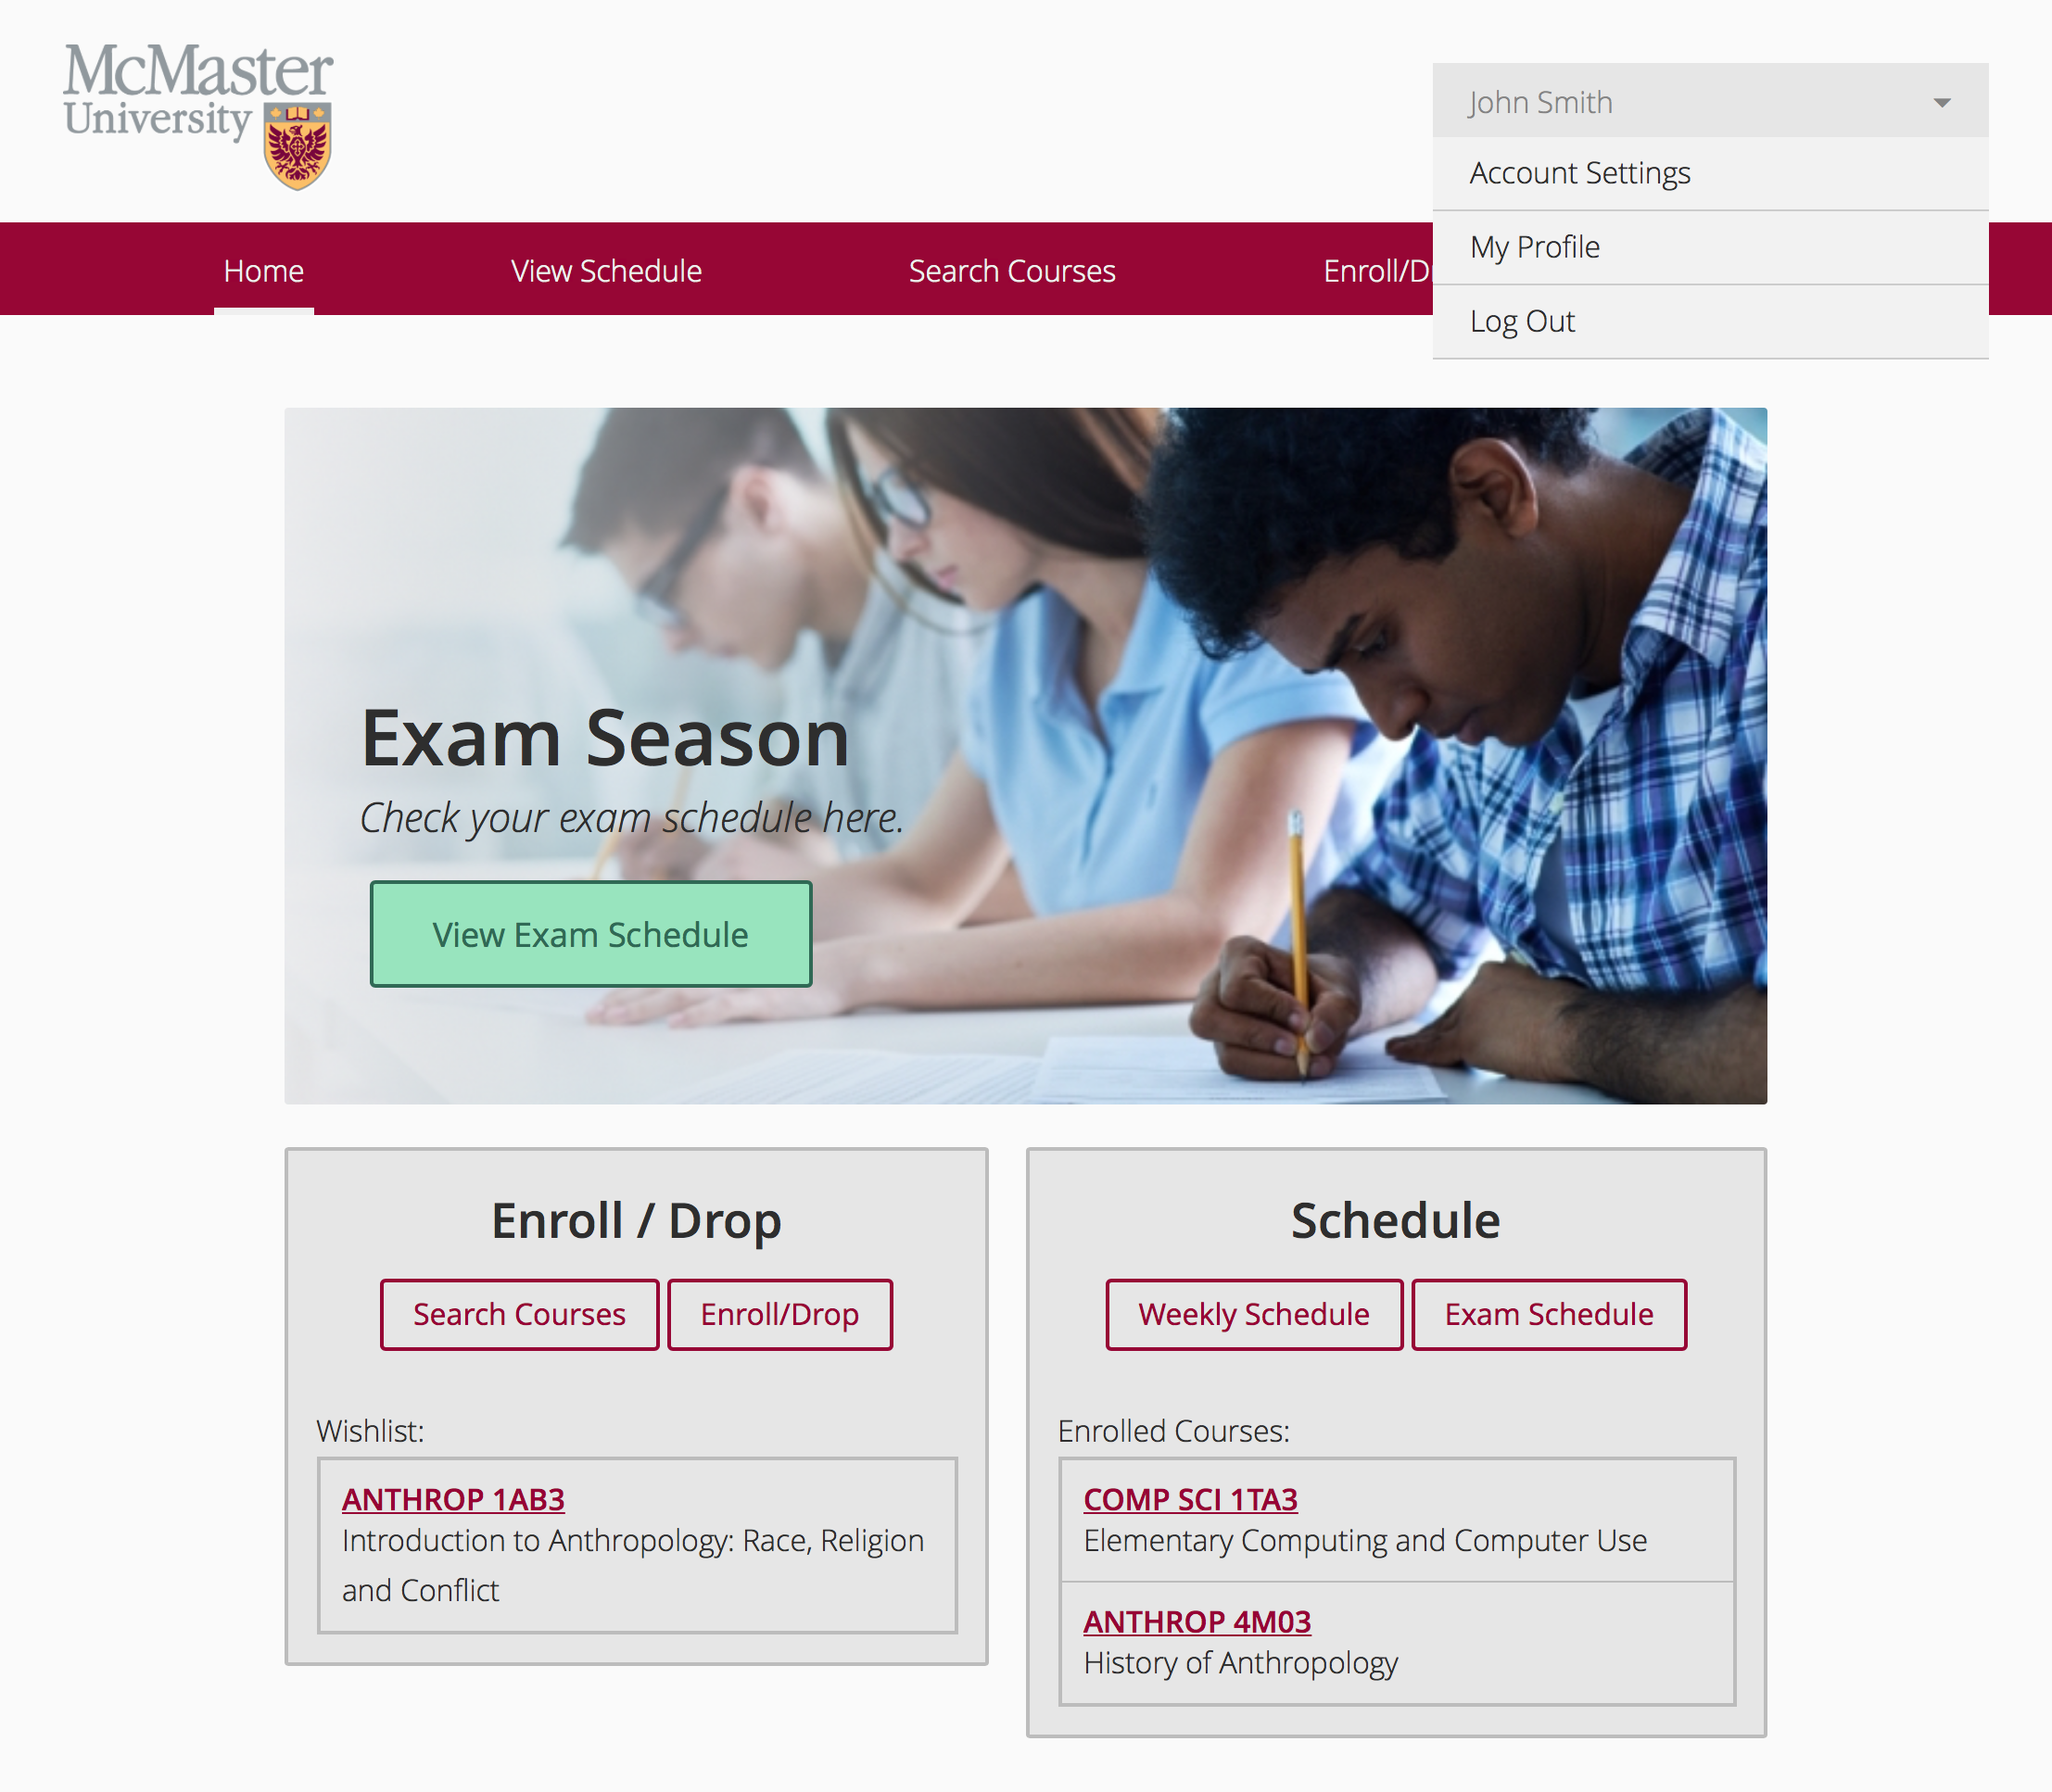
\includegraphics[width=\textwidth]{images/screen_home.png}}\\
    \Caption{New System Screenshot -- Home Page}
\end{figure}
\begin{figure}[h]
    \centering
    \fbox{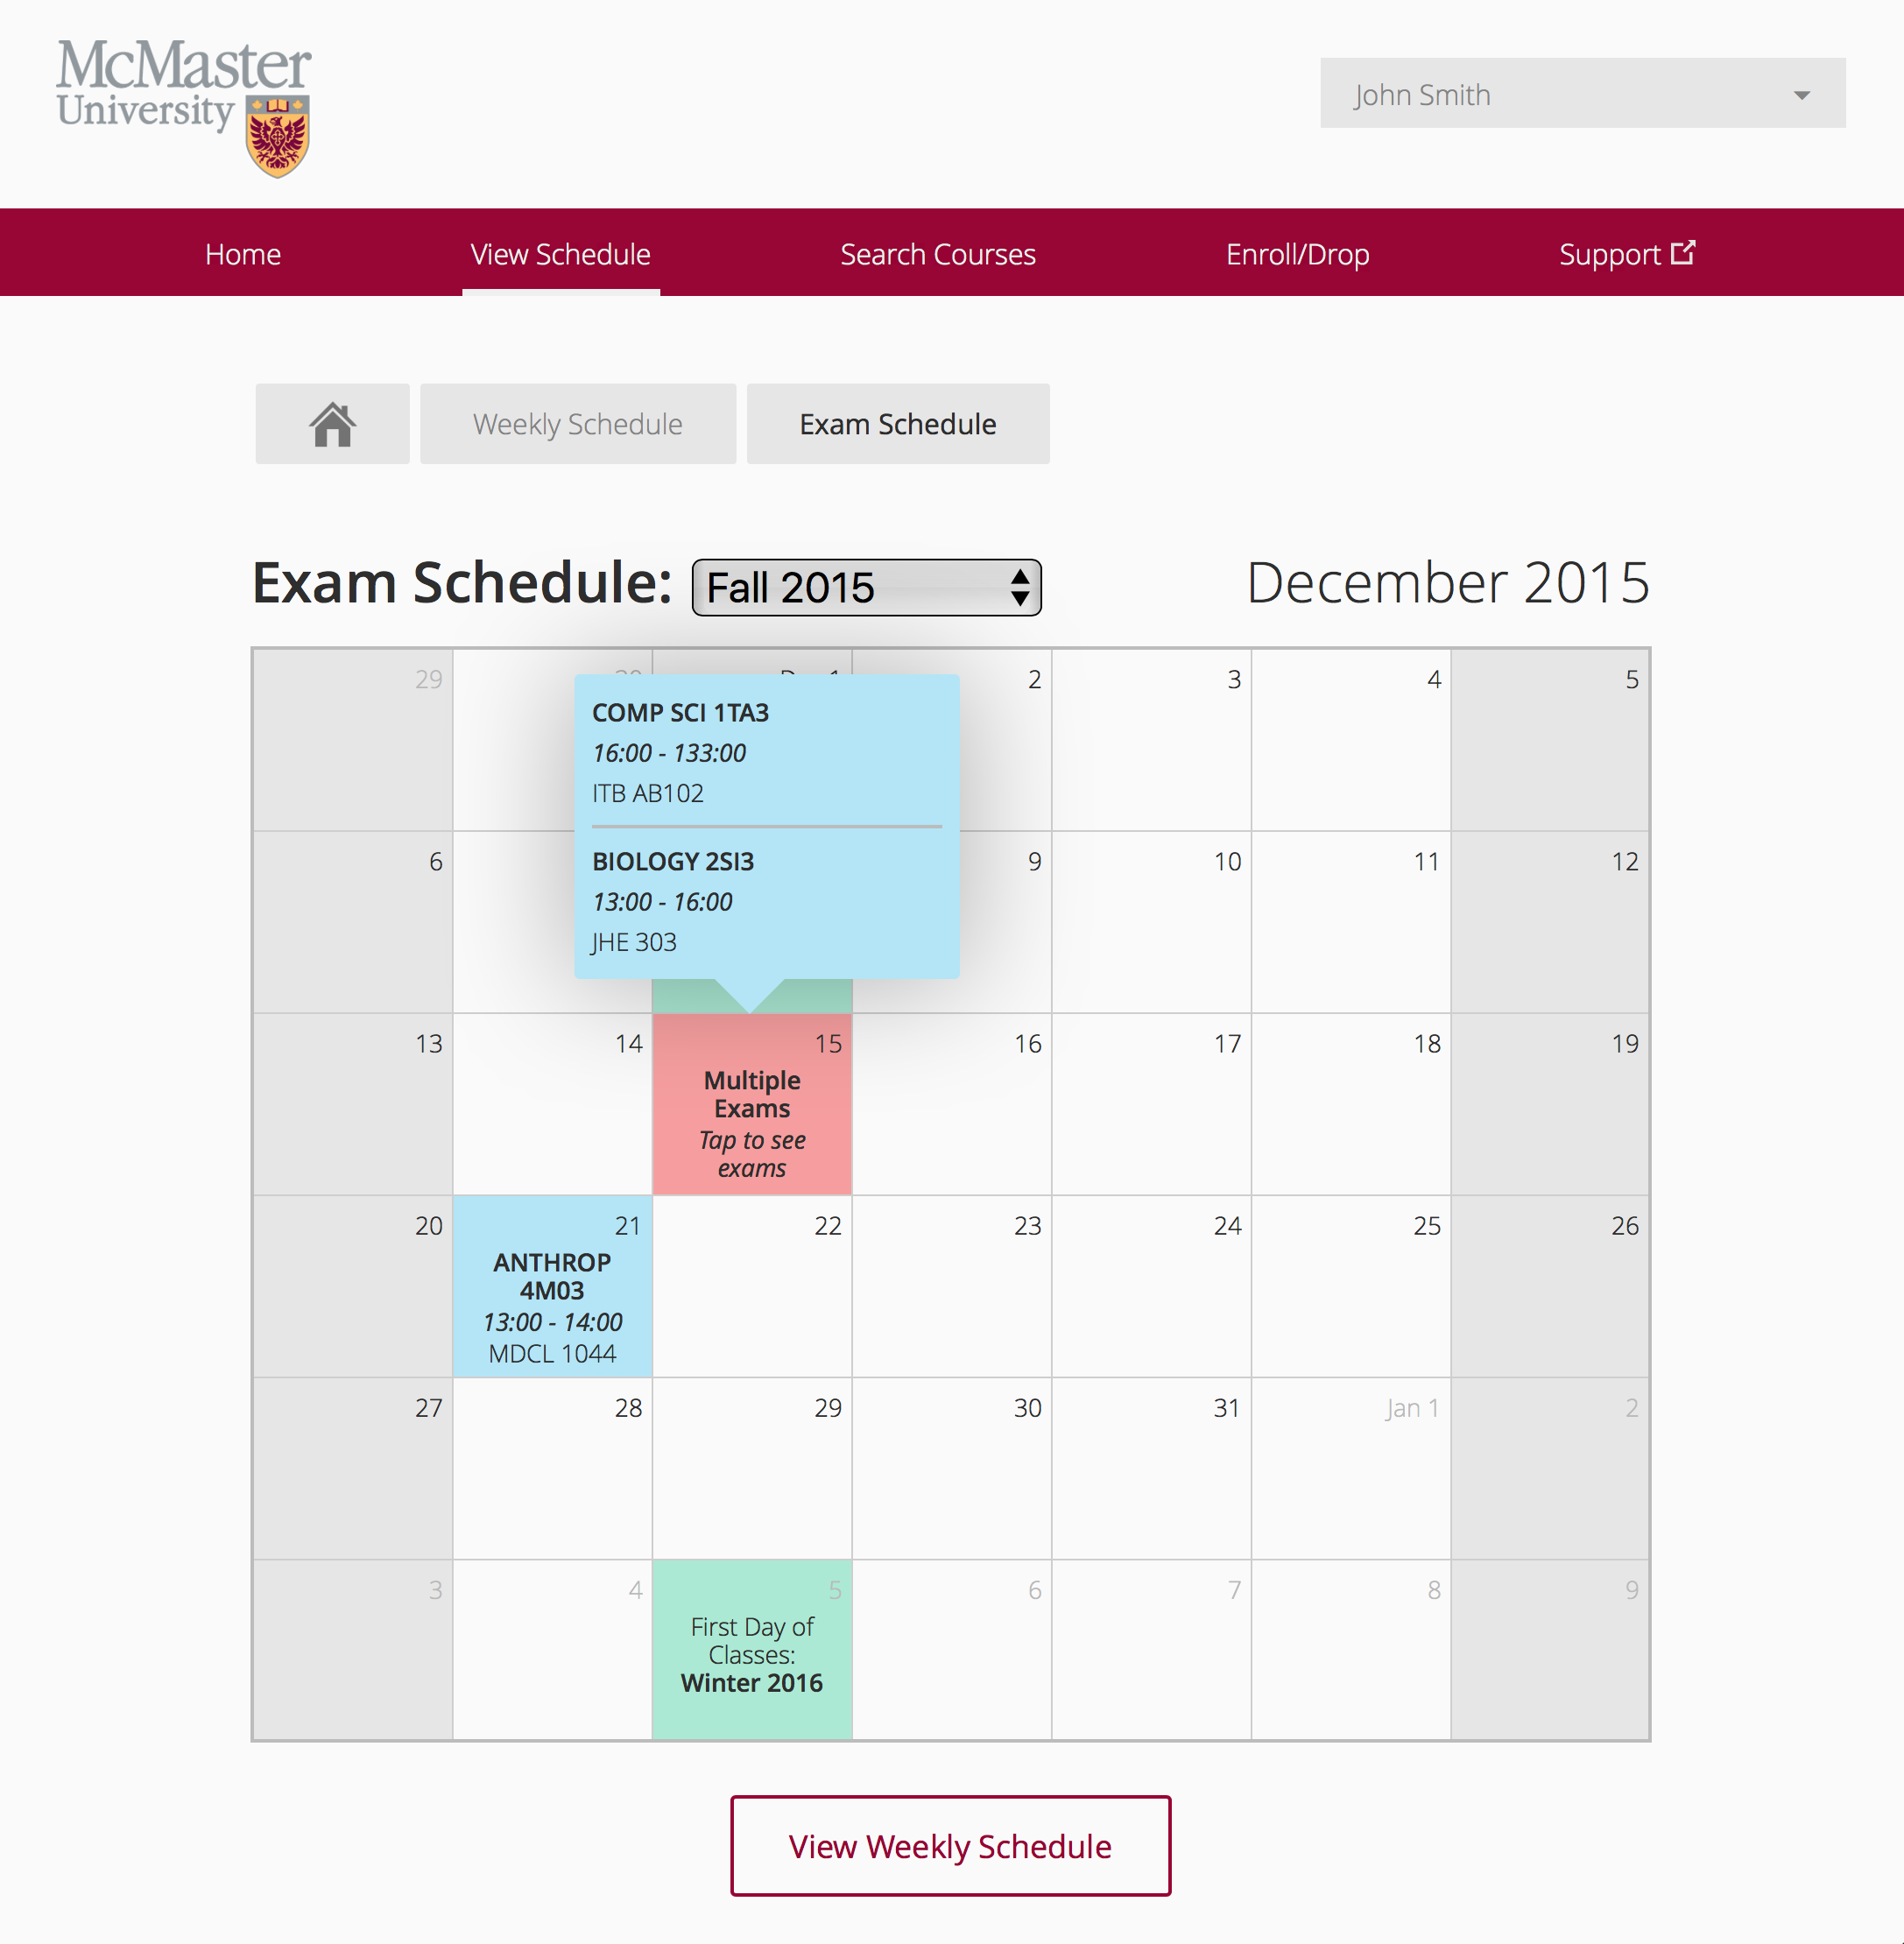
\includegraphics[width=\textwidth]{images/screen_exam.png}}\\
    \Caption{New System Screenshot --  Exam Schedule}
\end{figure}

\begin{figure}[h]
    \centering
    \fbox{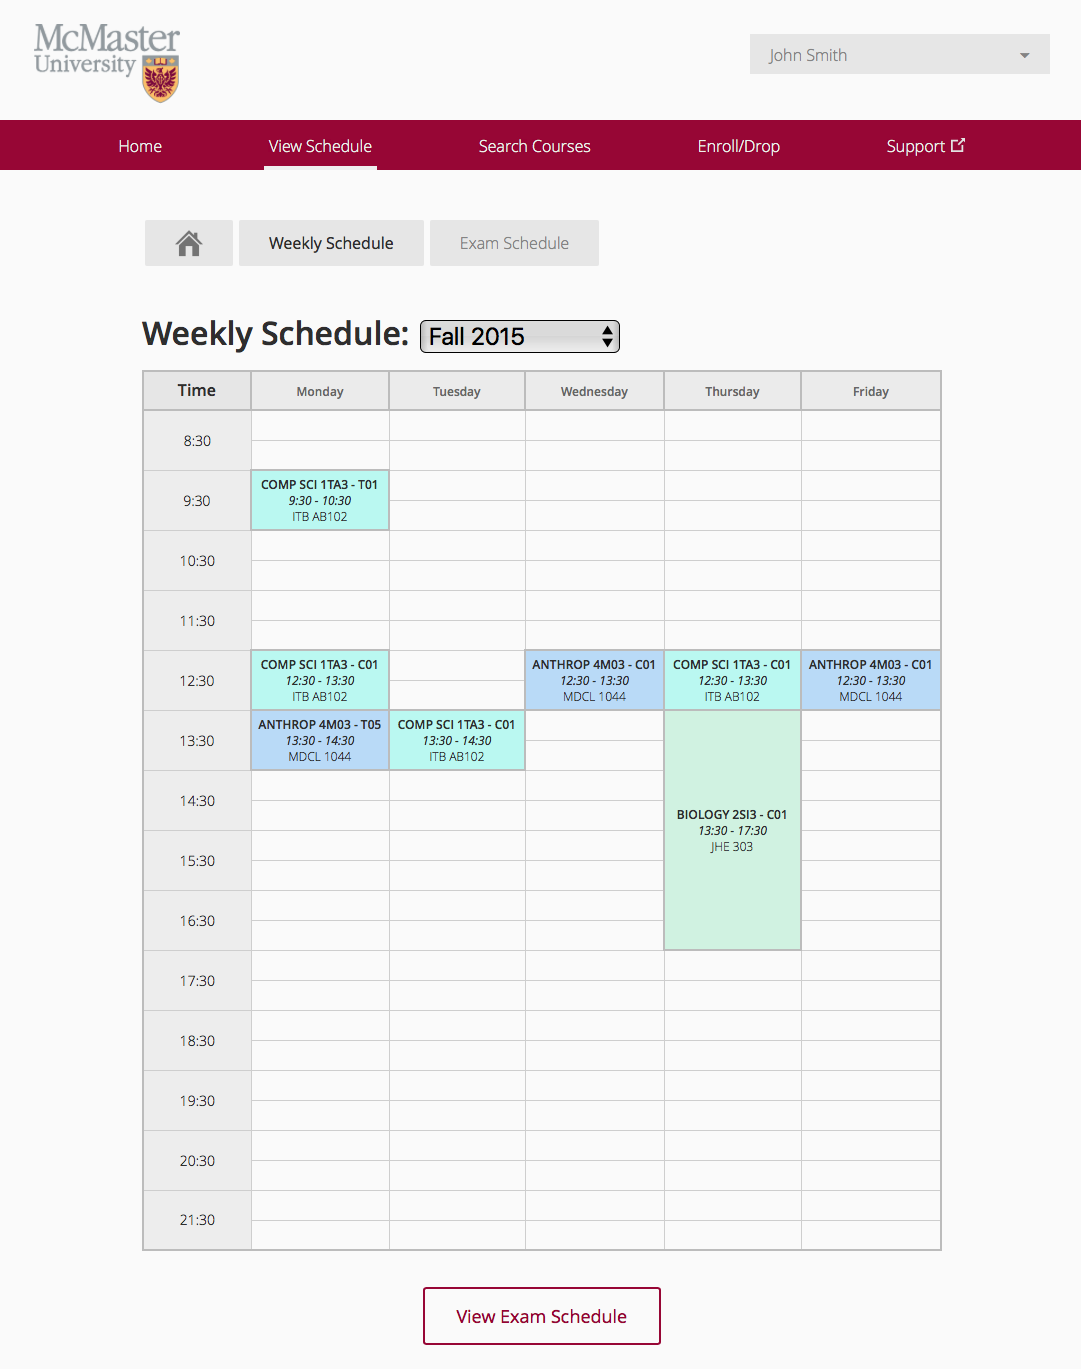
\includegraphics[width=\textwidth]{images/screen_weekly.png}}\\
	\Caption{New System Screenshot -- Weekly Schedule}
\end{figure}

\begin{figure}
    \centering
	\fbox{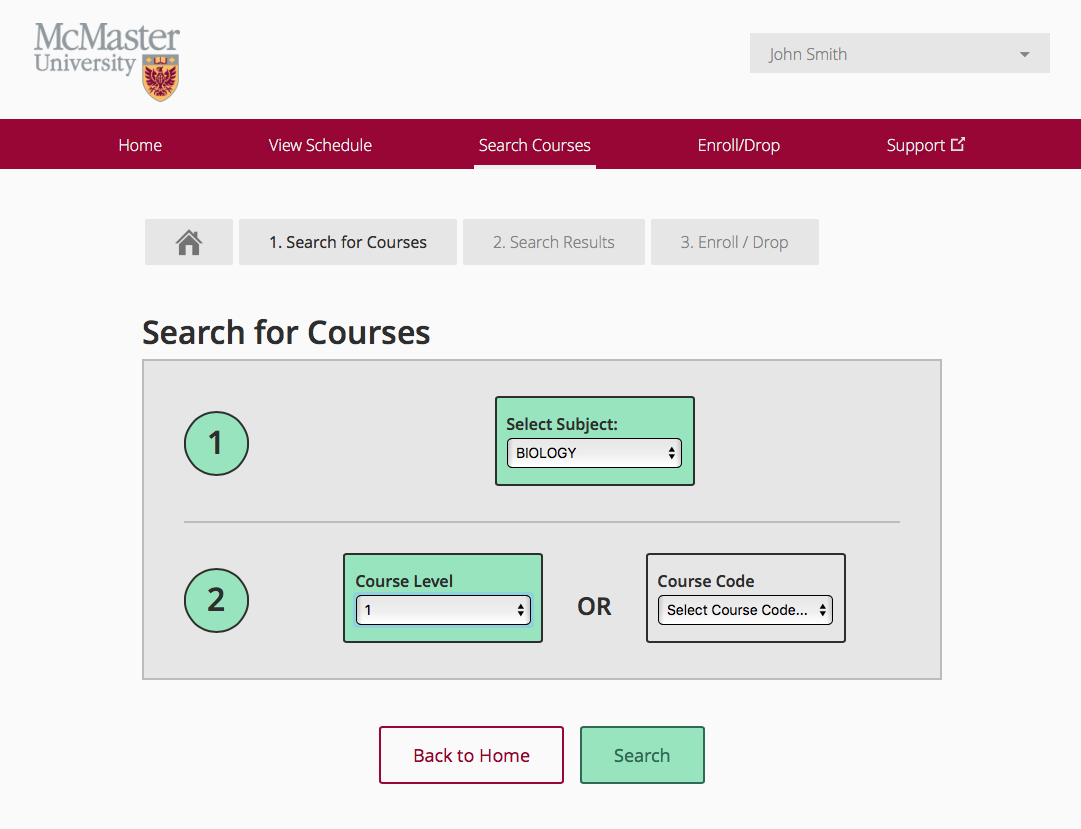
\includegraphics[width=\textwidth]{images/screen_criteria.png}}\\
	\Caption{New System Screenshot -- Search Criteria Page}
\end{figure}

\begin{figure}
    \centering
    \fbox{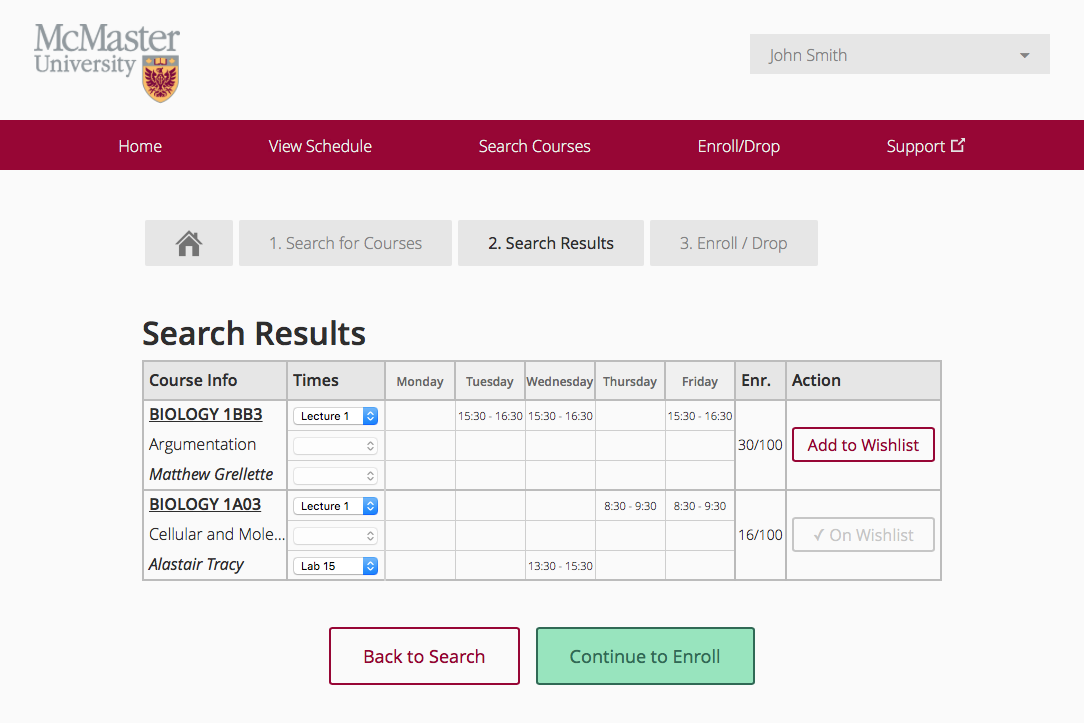
\includegraphics[width=\textwidth]{images/screen_results.png}}\\
    \Caption{New System Screenshot -- Search Results Page}
\end{figure}

\begin{figure}[h]
    \centering
    \fbox{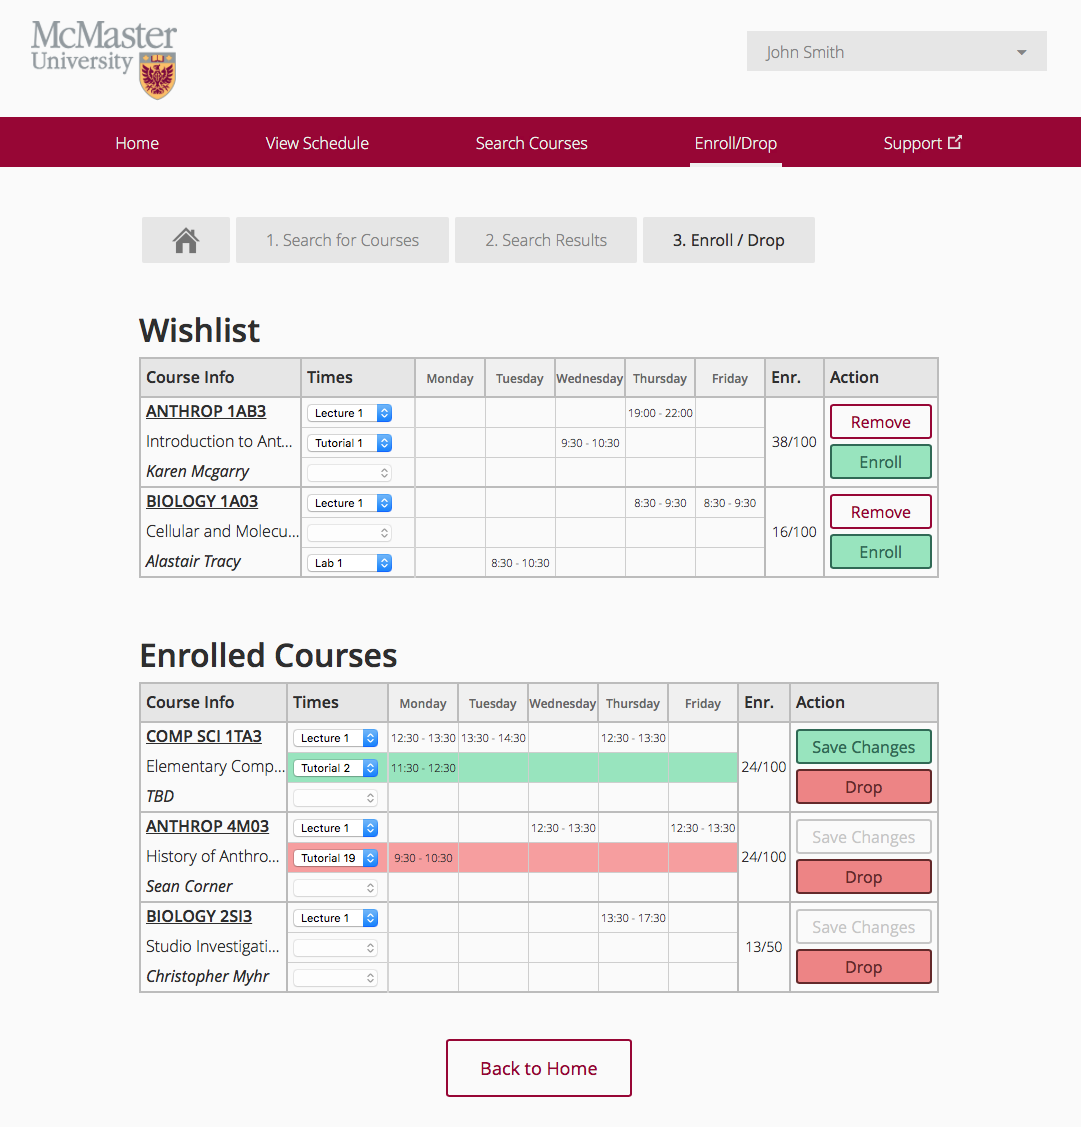
\includegraphics[width=\textwidth]{images/screen_enroll.png}}\\
    \Caption{New System Screenshot --  Enroll from Wishlist Page}
\end{figure}


\end{document}
